\chapter{System Modelling and Implementation} \label{ch:modelling}

The previous chapter introduced the biological and neuromorphic principles that are the foundations of this project. This chapter describes how those principles were converted into an implementable model for three-dimensional echolocation. The emphasis is not on reproducing every anatomical detail of a bat's auditory system, but on extracting the functional computations that appear useful for an engineered localisation system.

The final model follows a bottom-up design philosophy. Each major biological subsystem was first reduced to a computational role, then tested in isolation before being connected into a full pipeline. This led to a hybrid architecture. Most of the sensory pathways are fixed, interpretable, and hand-designed from biological principles, while a small trainable spiking readout was added at the end to learn residual context-dependent corrections. This is a deliberate compromise. A fully hand-designed model is easy to interpret but struggles when cues interact in full 3D. A fully trained black-box model can fit these interactions, but obscures the mechanism. The model developed here attempts to keep the pathway computations explicit while allowing limited training where biological integration would also be expected. This also lays the foundation for future work, which can use an expanded trainable model, using the results found from this project's model to make targeted training rather than a black-box approach.

\section{Modelling Methodology}

The modelling process used throughout the project was iterative rather than monolithic. Each stage was developed by following a similar sequence:
\begin{enumerate}
    \item identify the biological mechanism and its likely computational purpose,
    \item replace the detailed anatomy with the simplest useful mathematical abstraction that remains biologically grounded,
    \item test that abstraction in a small, isolated mini-model,
    \item integrate the abstraction into the relevant pathway,
    \item measure the resulting failure modes and add complexity only when needed.
\end{enumerate}

This process was important because the biological system is much more complex than the model can or should be. The cochlea, cochlear nuclei, lateral lemniscus, inferior colliculus, auditory cortex, and superior colliculus all contain many cell types and recurrent loops. Modelling all of these directly would produce a large simulation with many unconstrained parameters. Instead, the model treats biological structures as functional blocks. For example, the cochlea is treated as a tonotopic filterbank and spike encoder, the VCN as an onset-sharpening stage, the IC as a coincidence and population-code construction stage, and the SC as a population readout.

The main design tradeoff was therefore between biological detail and engineering clarity. Wherever the biology offered a clear algorithmic principle, that principle was retained. Examples include Jeffress-style timing comparison, LSO/MNTB excitation-inhibition comparison, DCN-like spectral notch detection, and attractor-based population stabilisation. Wherever the biology was poorly constrained or too detailed for the scope of the project, a simpler abstraction was used. For instance, the true cochlear mechanics were replaced by an IIR filterbank, the detailed VCN/VNLL latency-compensation circuitry was replaced by onset detection and a calibrated latency vector, and the final cortical integration was represented by a small trainable SNN rather than a full auditory cortical model.

This modelling strategy also separates two kinds of performance. The fixed pathway model tests whether the biological abstractions contain enough information to solve the task. The trainable readout tests whether remaining systematic errors are due to missing sensory information or simply imperfect calibration between available cues. This separation makes the model more interpretable than an end-to-end trained system.

\section{Full System Overview}

The final model estimates a target's distance, azimuth, and elevation from a single active echolocation call. The input scene is specified by spherical coordinates:
\begin{equation}
    (r, \theta, \psi),
\end{equation}
where $r$ is distance, $\theta$ is azimuth, and $\psi$ is elevation. These coordinates define the acoustic echo received at the ears. The model then processes the echo through three parallel pathways, each designed around a different localisation cues, as discussed in Chapter \ref{ch:background}.

The high-level computational flow is shown in Figure \ref{fig:top_level_system_block}.

\begin{figure}[htbp]
    \centering
    \begin{subfigure}{\textwidth}
        \centering
        \begin{tikzpicture}[
            % Define professional block styles
            block/.style={
                draw, 
                rectangle, 
                minimum height=1.2cm, 
                minimum width=2.6cm, 
                rounded corners=3pt, 
                line width=0.8pt,
                align=center,
                fill=white,
                font=\small\sffamily\bfseries
            },
            % Define special style for the parallel track components
            pathway/.style={
                block,
                minimum width=3.2cm,
                fill=gray!5 % Subtle shading to group them visually
            },
            % Clean arrow style matching journal standards
            arrow/.style={
                -{Stealth[scale=1.2]},
                line width=0.8pt
            }
        ]
        
        % --- Node Placements ---
        
        % External Motor / Environment Layer
        \node (siggen) [block] {Signal\\Generation};
        
        % 1. Input Stage (Positioned directly below Signal Generation)
        \node (signal) [block, below=1.6cm of siggen] {Received\\Echo};
        
        % 2. Frontend Pre-processing
        \node (cochlea) [block, right=1.0cm of signal] {Cochlea};
        
        % 3. Parallel Processing Pathways 
        \node (azimuth) [pathway, right=1.4cm of cochlea] {Azimuth\\Pathway};
        \node (distance) [pathway, above=0.6cm of azimuth] {Distance\\Pathway};
        \node (elevation) [pathway, below=0.6cm of azimuth] {Elevation\\Pathway};
        
        % 4. Output / Integration Stage
        \node (readout) [block, right=1.4cm of azimuth] {Combined\\Readout};
        
        % --- Signal Routing Arrows ---
        
        % New Connections from Signal Generation
        \draw [arrow] (siggen) -- node[right, midway, font=\scriptsize\sffamily\bfseries] {Environment} (signal);
        
        % L-shaped routing for Corollary Discharge over the top of the frontend
        \draw [arrow] (siggen.east) -| node[above, pos=0.4, font=\scriptsize\sffamily\bfseries] {Corollary Discharge} (distance.north);
        
        % Main entry paths
        \draw [arrow] (signal) -- (cochlea);
        
        % Demultiplexing split from Cochlea out to the three parallel paths
        \draw [arrow] ([yshift=0.2cm]cochlea.east) -- ++(0.4,0) |- (distance.west);
        \draw [arrow] (cochlea.east) -- (azimuth.west);
        \draw [arrow] ([yshift=-0.2cm]cochlea.east) -- ++(0.4,0) |- (elevation.west);
        
        % Multiplexing merge from the paths back down into the Readout matrix
        \draw [arrow] (distance.east) -- ++(0.4,0) |- ([yshift=0.2cm]readout.west);
        \draw [arrow] (azimuth.east) -- (readout.west);
        \draw [arrow] (elevation.east) -- ++(0.4,0) |- ([yshift=-0.2cm]readout.west);
        
        \end{tikzpicture}
    \end{subfigure}
    \caption{Top-level computational architecture of the neuromorphic 3D localisation pipeline. Active vocalisation triggers an internal corollary discharge to prime the distance pathway's temporal arithmetic, while the acoustic emission interacts with the environment to form the incoming sensory signal.}
    \label{fig:top_level_system_block}
\end{figure}

The initial signal generated produced a CD spiking efference copy by design, and the acoustic waveform is simulated through a virtual environment. This is received and encoded into spikes by the cochlea, which sends multiple channels (a frequency bank) of spike trains to three separate pathways. We will refer to this collection of spiking signals as the cochlear spike raster, or CSR.

Each pathway processes the CSR in parallel to the others, and produces both a raw population code and a decoded coordinate. This population code refers to the spiking activity of each neuron in the final population of neurons at the end of the pathway. The population code is important because it contains uncertainty and ambiguity that is lost in a single scalar prediction. 

Initially, the readouts from these pathways were kept independent, each with an independent parallel SC model, which will act as our readout. We will explore the different SC models tested and discuss the benefits of each. The final model uses a CANN model at the end of each pathway, and then uses a trainable SNN ``fusion'' combined readout. This final trainable readout receives the raw pathway populations as well as the CANN-decoded coordinate estimates.

This section will discuss the workings of the final model, as well as some of the key experiments and testing done to develop it, highlighting and motivating key design choices.

\section{Neuron Testing and Coincidence Detection}

Before the final architecture was assembled, several smaller models were built to understand and test the fundamental building blocks of the model. These experiments were not intended to be final localisation systems. Their purpose was to establish which neural mechanisms should be used in the full model and which could be simplified. Whilst many of these were done, the most fundamental experiment was testing the coincidence detection mechanism, as this underpins many of the pathway computations.

\subsection{Single Spike Coincidence Detecton Test}

Three distinct neural coincidence detectors were tested, each based on a different neuron type. LIF neurons and RF neurons were used for the first two, with a binary-based system tested as a control and possible optimised option. These were tested on a simple distance-based model, with a single spike input (the CD) and a returned delayed spike input (the echo).  These were fed into a bank of coincidence detectors, using each neuron as its base. The configuration of the experiment is shown in table \ref{tab:simulation_parameters}.

\begin{table}[htbp]
\centering
\caption{Simulation and Distance Pathway Benchmark Configurations}
\label{tab:simulation_parameters}
\begin{tabular}{l r}
\hline
\textbf{Parameter} & \textbf{Value} \\ \hline
Sample rate & 64,000~Hz \\
Speed of sound & 343.0~m/s \\
Distance range & 0.25 $\rightarrow$ 5.0~m \\
Delay lines & 160 \\
Time steps & 2,010 \\ \hline
\end{tabular}
\end{table}

The LIF and RF neurons functioned as described in Chapter \ref{ch:background}, and the binary coincidence detection was effectively an AND gate of the time vectors of CD efference copy and the echo.

\begin{figure}[h]
    \centering
    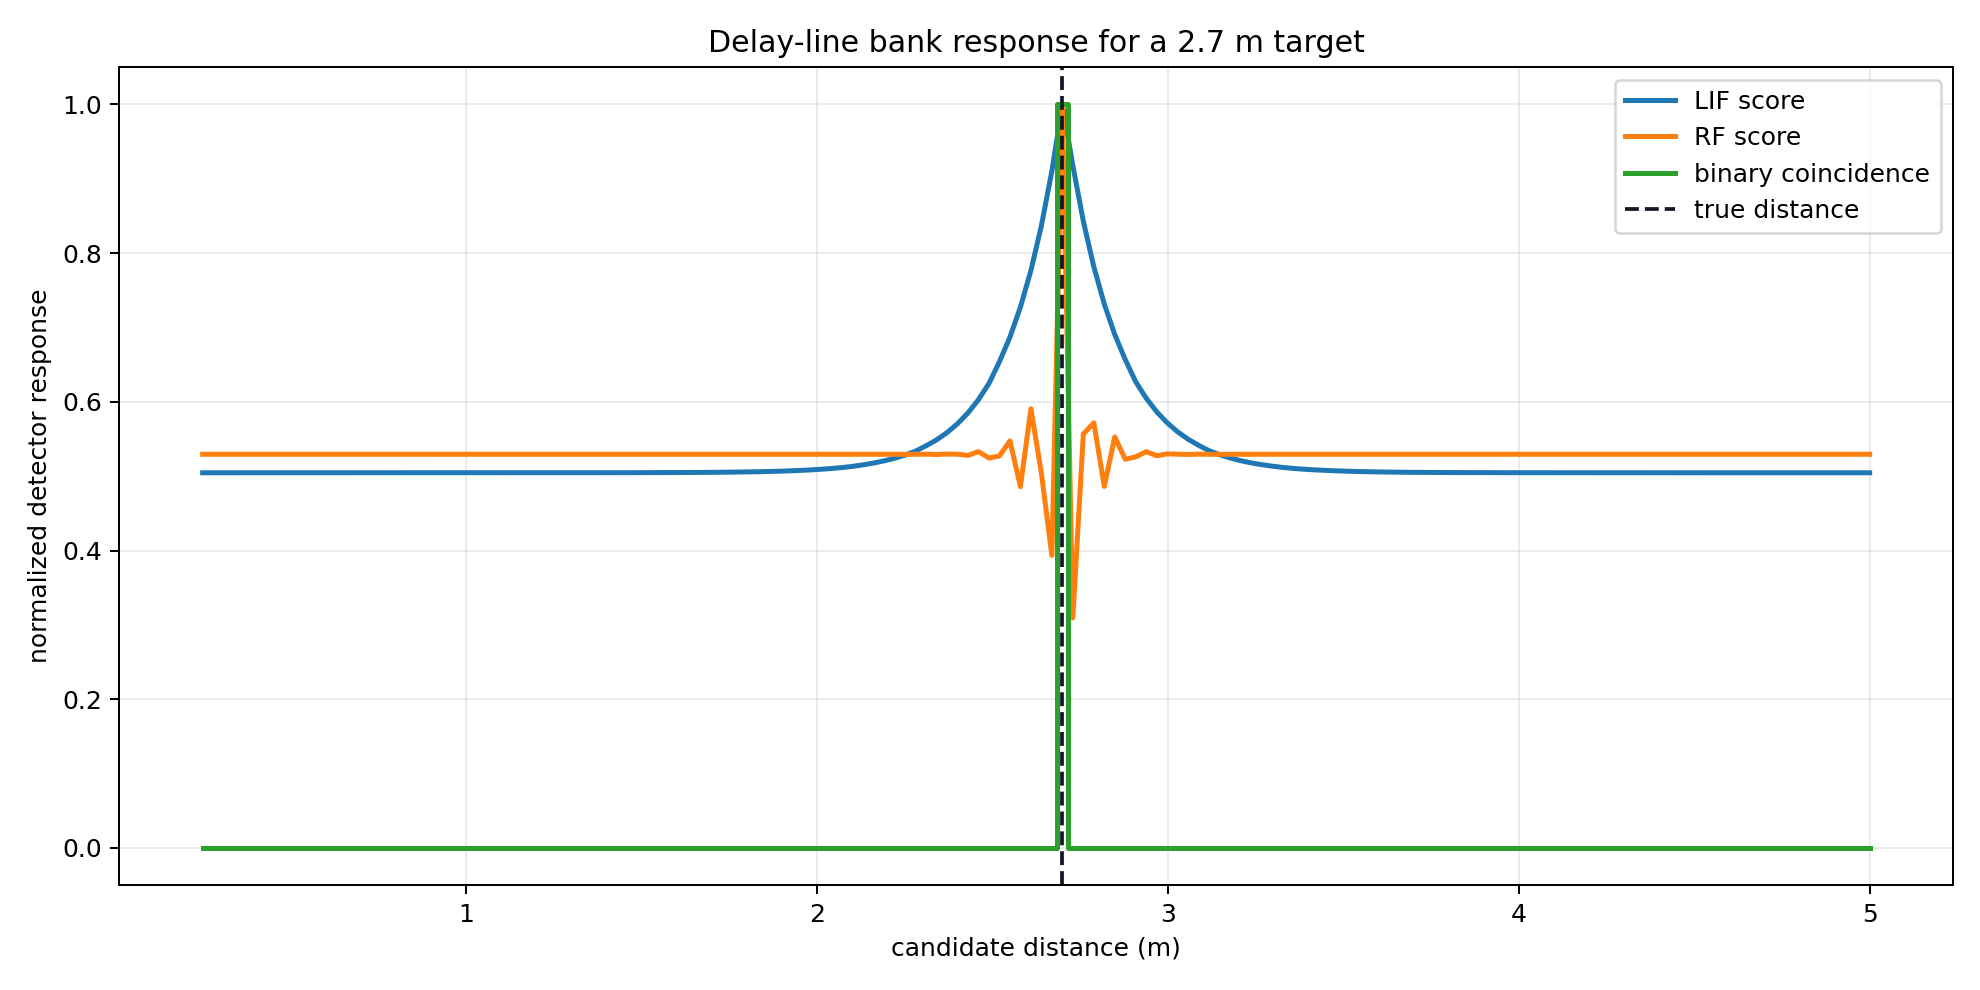
\includegraphics[width=0.7\textwidth]{3_Modelling/coincidence_detection/responses.png}
    \caption{Example responses of the tested coincidence detectors. The plot shows a single target at 2.7m. The matched delay line peaks at the correct distance.}
    \label{fig:responses}
\end{figure}

\subsection{Noise and Single Channel Results}

When restricted to a single processing channel, all three coincidence detectors were highly vulnerable to environmental noise. This noise was modelled simply as three extra spurious spikes with random delays uniformly sampled across the time after the primary echo to the end of the simulation. The results of the clean and noisy experiments are shown in Table \ref{tab:spiking_input_error_metrics}.

\begin{table}[htbp]
\centering
\caption{Spiking Input Benchmark Performance: Clean vs. Added Noise Conditions}
\label{tab:spiking_input_error_metrics}
\small
\begin{tabular}{l l r r r r r}
\hline
\textbf{Condition} & \textbf{Detector} & \textbf{MAE (cm)} & \textbf{RMSE (cm)} & \textbf{Runtime (ms)} \\ \hline
Clean & LIF & 0.77 & 0.89 &  1.111 \\
              & RF  & 2.20 & 3.06 & 1.264 \\
              & Binary & 0.77 & 0.89  & 0.494 \\ \hline
Added noise   & LIF & 52.47 & 111.88  & 5.407 \\
              & RF  & 63.55 & 122.73 & 8.172 \\
              & Binary & 96.22 & 149.95 & 2.777 \\ \hline
\end{tabular}
\end{table}

Binary detectors suffer from catastrophic omissions due to strict hard-threshold clipping, while RF detectors generate spurious side-lobes from random phase alignments with white noise. LIF primitives perform marginally better due to their soft exponential decay profile, but single-channel processing remains fundamentally unviable for robust distance estimation.

\subsection{Adding Frequency Channels}

A multi-channel FM-sweep was then introduced. These signals are shown in Figure \ref{fig:frequency_channels}.

\begin{figure}[h]
    \centering
    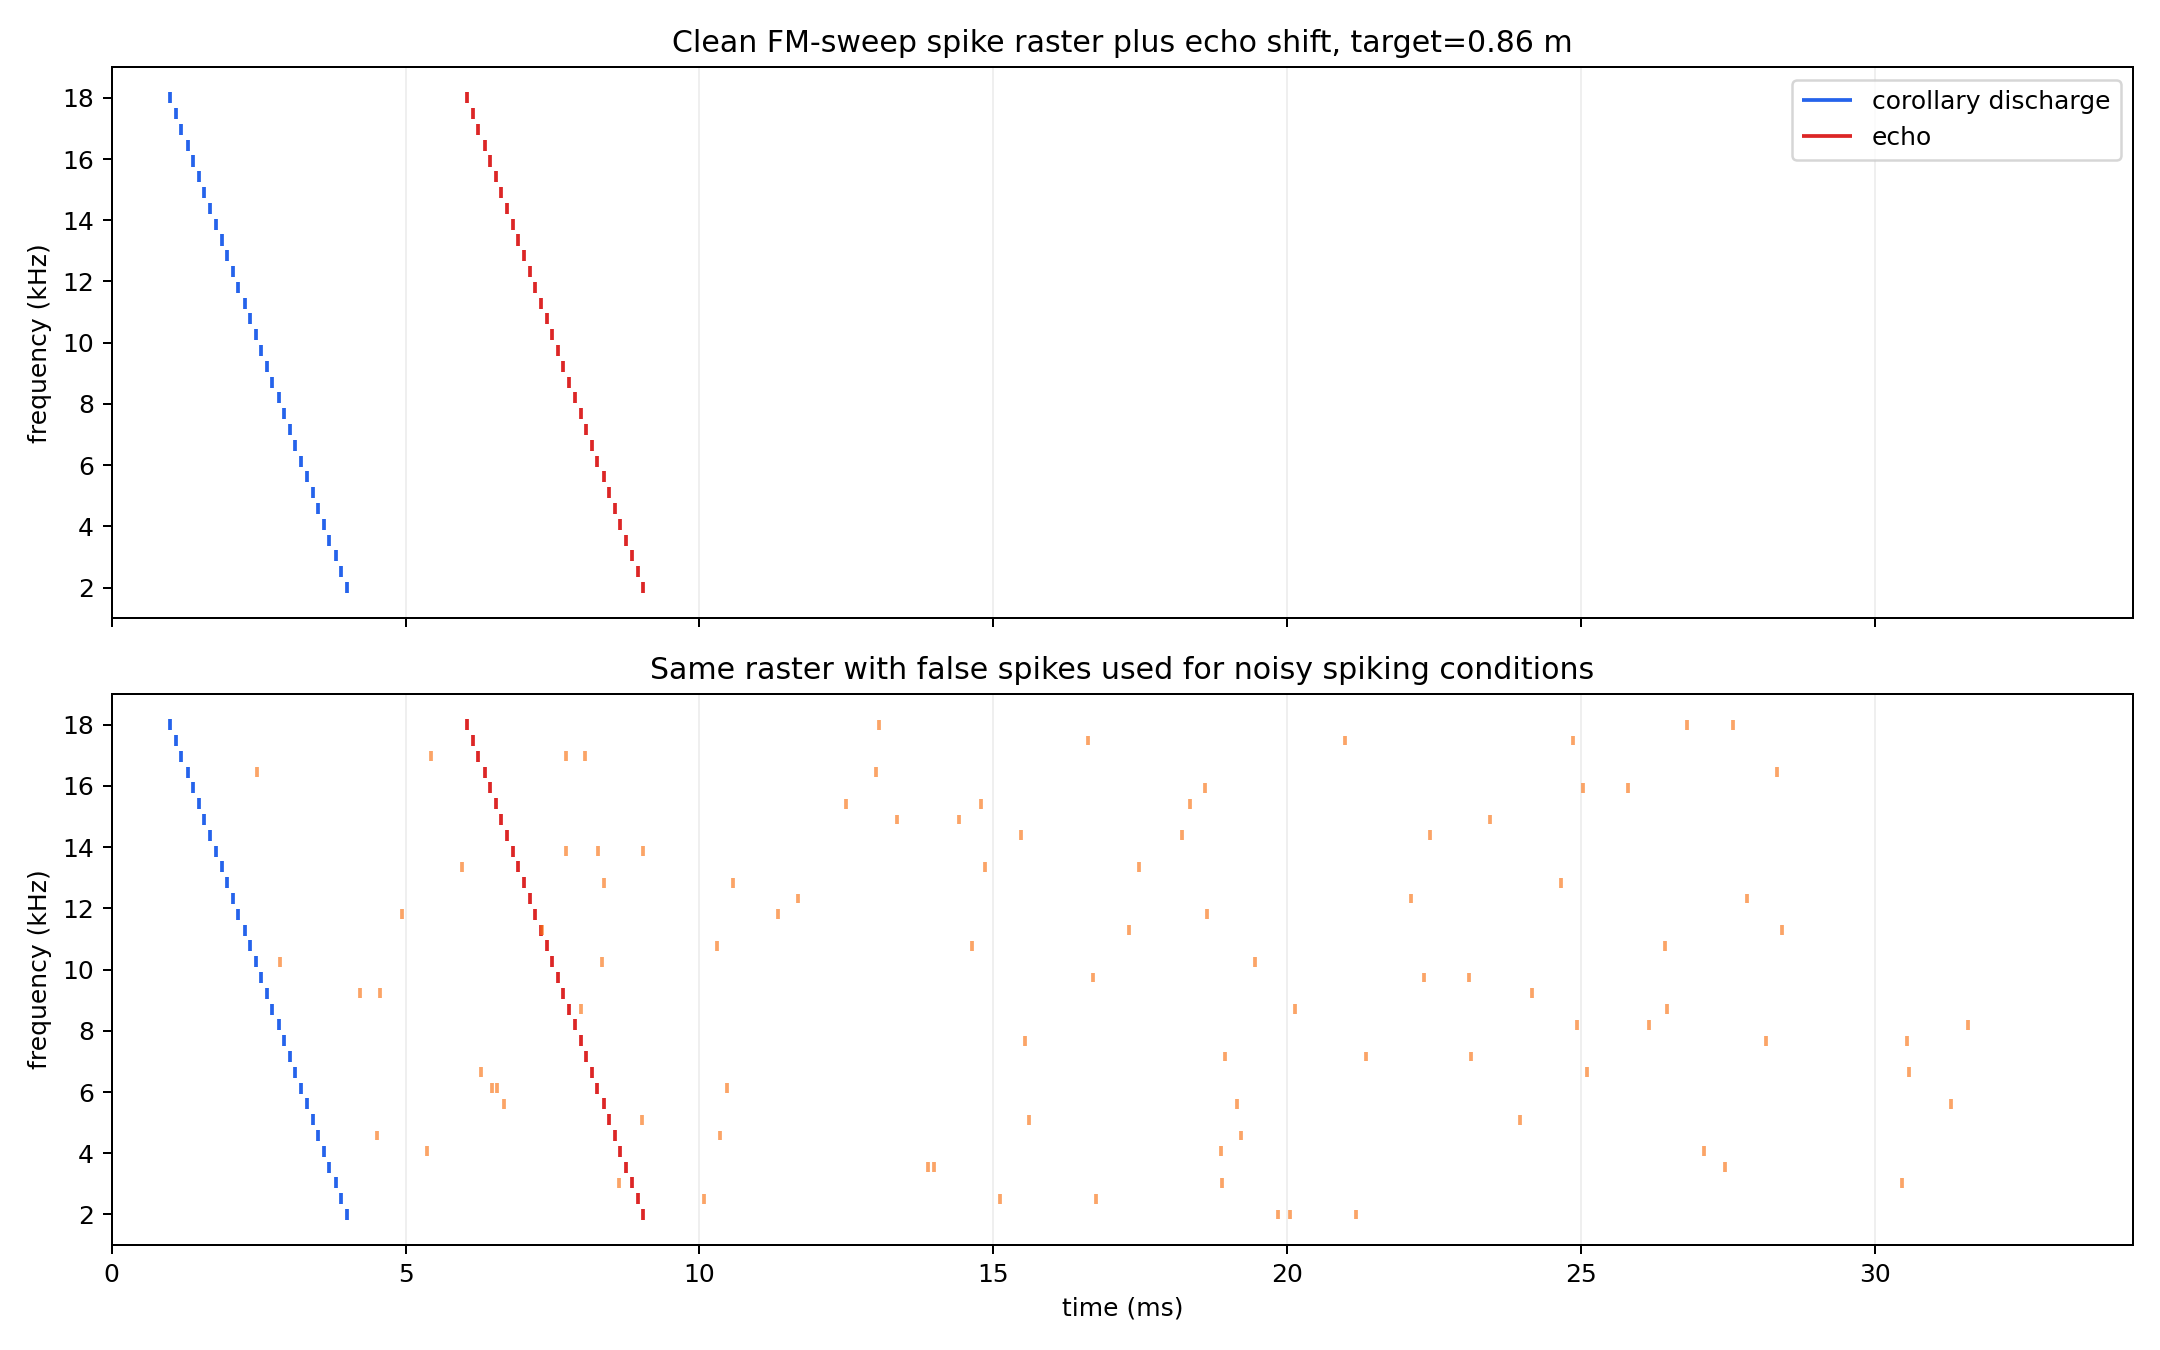
\includegraphics[width=0.7\textwidth]{3_Modelling/coincidence_detection/frequency_channels.png}
    \caption{The clean and noisy CD and echo spiking signals}
    \label{fig:frequency_channels}
\end{figure}

By cross-correlating a 32-channel swept corollary discharge reference against the incoming echo spikes, the network exploits tonotopic (spatial mapping of sound frequencies) redundancy. Because isolated false spikes are independent across frequency bands, they fail to form a coherent alignment vector across channels. When these per-channel alignment scores are averaged, the true target delay emerges as a reinforced global maximum, compressed back to sub-centimeter mean absolute error (MAE). These results are shown in Table \ref{tab:sweep_spiking_error_metrics}. Not only does the frequency channel reduce the error, but the added error from noise disappears entirely. 

\begin{table}[htbp]
\centering
\caption{FM-Sweep Spiking Input Benchmark Performance: Clean vs. Added Noise.}
\label{tab:sweep_spiking_error_metrics}
\small
\begin{tabular}{l l r r r}
\hline
\textbf{Condition} & \textbf{Detector} & \textbf{MAE (cm)} & \textbf{RMSE (cm)} & \textbf{Runtime (ms)} \\ \hline
Clean perfect & LIF detector & 0.77 & 0.89 & 45.927 \\
              & RF detector  & 2.20 & 3.06 & 66.351 \\
              & Binary detector & 0.79 & 0.92 & 16.165 \\ \hline
Added noise   & LIF detector & 0.77 & 0.89 & 200.981 \\
              & RF detector  & 2.20 & 3.06 & 300.766 \\
              & Binary detector & 0.79 & 0.92 & 55.673 \\ \hline
\end{tabular}
\end{table}

\subsection{Design Choices}

This experiment led to a few key design choice conclusions:

\begin{enumerate}
    \item \textbf{The necessity for a multi-channel system:} single-channel delay tracking is fundamentally brittle under realistic signal conditions ($\sim$50~cm MAE). Transitioning to an integrated 32-channel FM sweep compresses localisation error down to the same level as the clean experiment, proving that spatial tracking accuracy depends on cross-channel voting redundancy rather than single-unit precision. This makes the use of frequency channels not only essential for spectral cue computation, but for tonotopic redundancy and noise robustness.
    \item \textbf{The use of LIF neurons in the coincidence detector:} The LIF neuron was selected as the basis of all coincidence detectors. Despite its biological prominence in central auditory pathway modeling, the RF neuron was structurally unsuited for echo-ranging tasks. Further analysis was conducted into why this was, but essentially, the RF neuron is suited to rhythmic selectivity, rather than pure time differences. This means it punishes minor mistakes more than the LIF neuron. This could potentially be used with optimal tuning to create a more accurate system, however the brittle and phasic nature of the neuron left it undesirable to be the foundation of our computation.
    \item \textbf{Neuromorphic hardware implementation:} While the Binary primitive offers the smallest computational footprint (requiring only bitwise operations), the LIF primitive provides superior noise filtering in single-channel environments. It is also implementable on neuromorphic hardware, which was deemed important for this project, with the aim for the system being theoretically implementable on hardware in the future.
\end{enumerate}


\paragraph{A note on optimising coincidence detection.} It should also be noted that the runtime analytics have been included here. The binary system is by far the fastest system, and this was further optimised using an event coordinate system. This means that rather than saving to memory and analysing each time step, only the time steps where a spike occurs are saved and computed. This addition was show reduce runtime relative to the LIF-based system by over 99\%. This is however only a benefit for simulation, as it converts the model from a time step computing system to a layer by layer computation system, making it inherently uncausal. This would also not be implementable on neuromorphic hardware, and so the optimisation was not carried forward. Nevertheless, optimising the coincidence detector using a vectorised binary event-coordinate system may still be a useful finding which could be used to massively reduce runtimes should a future model be expanded or use training more heavily.

\section{Signals and Acoustic Environment}

Before we modelled the biological inference system, a virtual signal and environment were needed. These were modelled with the aim of simplified realism. 

\subsection{Designing the Signal}
Real bat call recordings were analysed for both an FM call (from the Pipistrellus pipistrellus bat) and a CF-FM call (from the Rhinolophus hipposideros bat) \cite{BatSounds}. The spectrograms of isolated example calls are shown in Figure \ref{fig:bat_calls}. These show ultrasonic calls with very different behaviours.

\begin{figure}[H]
    \centering
    
    % Panel A
    \begin{subfigure}[t]{0.45\textwidth}
        \textbf{\large A}\\[0.5ex]  % Forces the bold 'A' to the top left
        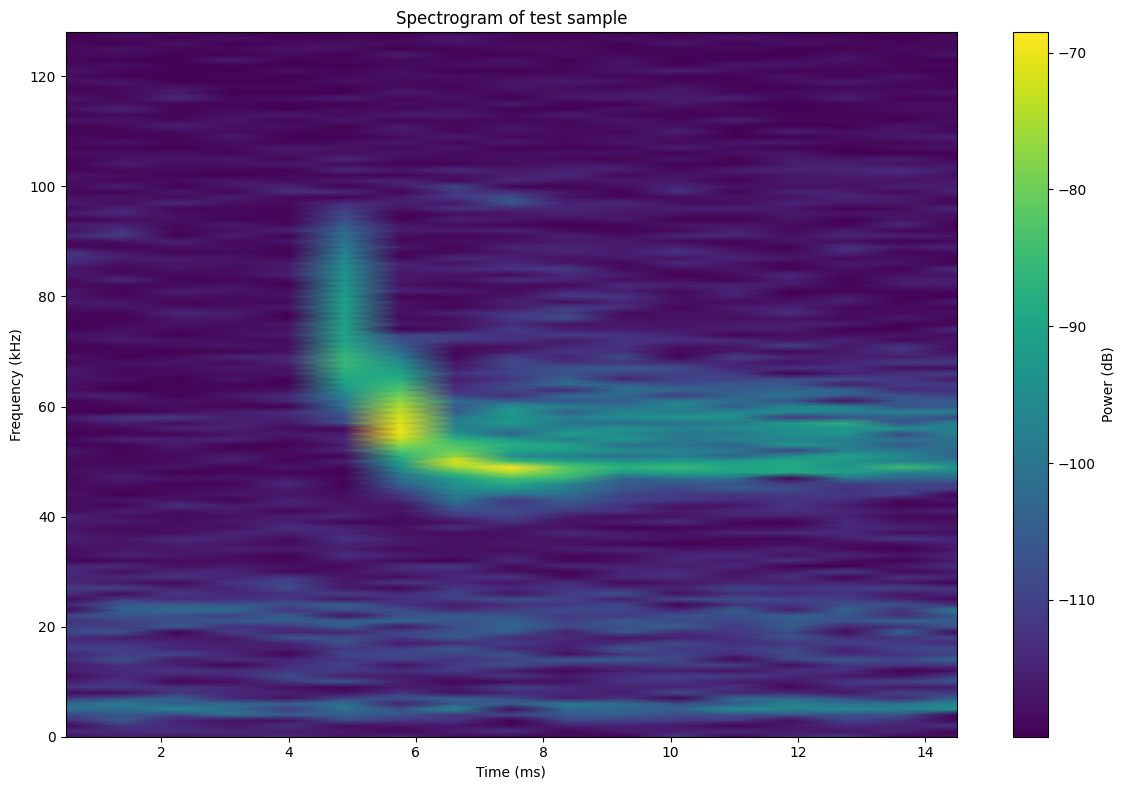
\includegraphics[height=4cm]{3_Modelling/signals/FM_call.png}
        \label{}
        \caption{}
    \end{subfigure}
    \hspace{0.1cm}
    % Panel B
    \begin{subfigure}[t]{0.45\textwidth}
        \textbf{\large B}\\[0.5ex]  % Forces the bold 'B' to the top left
        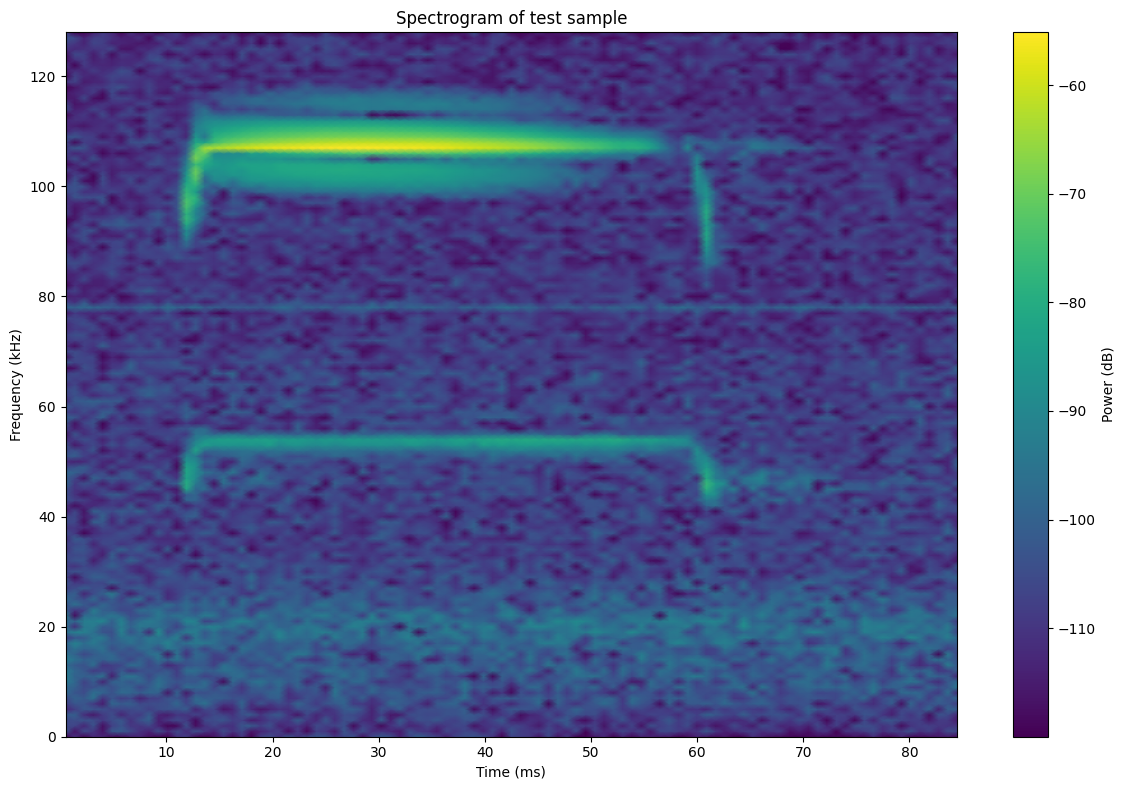
\includegraphics[height=4cm]{3_Modelling/signals/CF_call.png}
        \caption{}
        \label{}
    \end{subfigure}

    \caption{The Spectograms of real recorded bat calls of A: the Pipistrellus pipistrellus FM call, B: the Rhinolophus hipposideros CF call. Recordings from \cite{BatSounds}}
    \label{fig:bat_calls}
\end{figure}

Both calls were modelled and initially tested for their use in distance estimation. It was found that the FM call was much easier to use and work with, with the CF call returning negative distances at times, due to its long chirp time of over 40ms. Hence, an FM call was chosen for use.

The simulated emitted call was modelled as a Hann-windowed frequency-modulated chirp. In the main experiments, the chirp sweeps downward from $18$~kHz to $2$~kHz over $3$~ms at a sampling frequency of $64$~kHz. The use of lower frequencies than real microbat ultrasound was an intentional simplification. It reduced sample-rate requirements and keeps the model computationally manageable while preserving the key structure of the problem: a broadband time-varying signal whose echo can be matched against an internal reference. The modelled call is shown in Figure \ref{fig:modelled_call}.


\begin{figure}[h]
    \centering
    
\includegraphics[width=0.5\textwidth]{3_Modelling/signals/modelled_call.png}
    \caption{Amplitude-time plot and artificial spectrogram of modelled emitted signal. An artificial spectrogram was used to show the frequency sweep behaviour clearly, due to the limits of an STFT.}
    \label{fig:modelled_call}
\end{figure}

The instantaneous chirp can be written as:
\begin{equation}
    s(t) = A w(t)\sin\left(2\pi\left[f_0 t + \frac{1}{2}kt^2\right]\right),
\end{equation}
where $A$ is the transmitted amplitude, $w(t)$ is the Hann window, $f_0$ is the starting frequency, and $k$ is the sweep rate. The transmitted gain is treated as a $140$~dB call relative to an original $80$~dB reference convention. This was not intended as a precise acoustic calibration of a bat call, but provides a consistent amplitude scale for testing attenuation and noise.

\subsection{Modelling the Environment}

After the signal is emitted, it is sent through a virtual environment with multiple processing blocks. The overall transformation pipeline is shown in Figure \ref{fig:monaural_simulation_pipeline}.


\begin{figure}[htbp]
    \centering
    \begin{tikzpicture}[
        % Compact dimensions to ensure a clean horizontal fit on a single page
        block/.style={
            draw, rectangle, 
            minimum height=1.1cm, 
            minimum width=1.8cm, 
            rounded corners=3pt, 
            line width=0.8pt, 
            align=center, 
            fill=white, 
            font=\scriptsize\sffamily\bfseries
        },
        nobox/.style={
            rectangle, 
            minimum height=1.1cm, 
            minimum width=1.8cm, 
            align=center, 
            font=\scriptsize\sffamily\bfseries
        },
        arrow/.style={
            -{Stealth[scale=1.2]}, 
            line width=0.8pt
        }
    ]
    
    % ==================== LINEAR SIMULATION PIPELINE ====================
    \node (source) [nobox] at (0,0) {Source\\Signal};
    \node (delay)  [block, right=0.35cm of source] {Time\\Delay};
    \node (atten)  [block, right=0.35cm of delay]  {Distance\\Attenuation};
    \node (shadow) [block, right=0.35cm of atten]  {Head\\Shadow};
    \node (spec)   [block, right=0.35cm of shadow] {Spectral\\Filtering};
    \node (noise)  [block, right=0.35cm of spec]   {Noise\\Addition};
    \node (wave)   [nobox, right=0.35cm of noise]  {Received\\Waveform};

    % ==================== CONNECTIONS ====================
    \draw [arrow] (source) -- (delay);
    \draw [arrow] (delay)  -- (atten);
    \draw [arrow] (atten)  -- (shadow);
    \draw [arrow] (shadow) -- (spec);
    \draw [arrow] (spec)   -- (noise);
    \draw [arrow] (noise)  -- (wave);

    \end{tikzpicture}
    \caption{Monaural signal transformation pipeline demonstrating the sequential processing stages required to generate a localized acoustic waveform instance.}
    \label{fig:monaural_simulation_pipeline}
\end{figure}

\paragraph{Time Delay:} For a target at distance $r$, the dominant echo delay is approximately:
\begin{equation}
    \Delta t \approx \frac{2r}{c},
\end{equation}
where $c$ is the speed of sound. In the binaural simulator the path length is computed separately for each ear, so azimuth also creates a small interaural timing difference due to having slightly different path lengths. 

\paragraph{Attenuation:} Echo amplitude is attenuated using an inverse-square law:
\begin{equation}
    A_{\text{echo}} = \frac{0.7}{L^2}A_{\text{call}},
\end{equation}
where $L$ is the total acoustic path length. The constant $0.7$ represents a reflection/gain factor. It is a simplification of target reflectivity, atmospheric losses, and ear gain.

\paragraph{Head Shadow:} Azimuth was also encoded through a multiplicative head-shadow term. We did not model a full frequency-dependent HRTF, instead we applied a smooth left/right gain asymmetry, using equation \ref{eq:head_shadow}. This kept the binaural cue interpretable while still producing realistic ILD-like information.

\begin{equation}
    G_{\text{shadow}, i} = \exp\left( s_{\text{shadow}} \cdot \sin \theta \cdot \sigma_i \right)
\label{eq:head_shadow}
\end{equation}
where $s_{\text{shadow}}$ is a scalar head shadow intensity coefficient, $\theta$ is the acoustic azimuth angle, and $\sigma_i$ is the directional sign modifier designated for each side ($\sigma_{\text{L}} = 1, \sigma_{\text{R}} = -1$).

Spectral filtering is then done by the pinna. Noise is then added naively at the end of this pipeline to represent all noise in the system. This may not have been realistic, as environmental noise will be affected by the HRTF and the pinna, but it still tests the system's response to a noisy signal.

\subsection{Modelling the Pinna} 

The pinna performs spectral filtering, as discussed in Chapter \ref{ch:background}, which encodes information for elevation. This was simplified to a single sweeping `notch', with strong local attenuation at different frequencies based on the elevation. Three mechanisms were proposed for creating this notch: a negative Gaussian, an inverted Butterworth band-pass, and a comb filter. The comb filter was selected for its realism, representing interfering reflections from the pinna. Since a comb filter creates multiple notches, the model was designed such that there was a singular notch in the frequency range of the call (4kHz to 18kHz).

To model the comb filter, the received signal was combined with a delayed copy of itself:
\begin{equation}
    y(t)=x(t)+g x(t-\tau),
\end{equation}
where $g$ is the delayed-copy gain and $\tau$ is an elevation-dependent delay. The corresponding magnitude response of the transfer function is:
\begin{equation}
    |H(f)| = \frac{\sqrt{1+g^2+2g\cos(2\pi f \tau)}}{1+g}.
\end{equation}
Changing $\tau$ moves the spectral notches across frequency, creating a simplified pinna-like elevation cue, effectively encoding using the frequency of the first notch: 
\begin{equation}
    f_0 = \left. \frac{2m + 1}{2\tau} \right|_{m=0} = \frac{1}{2\tau}
\end{equation}
where $m$ is the notch number. From this we can also see that the second notch is three times the frequency of the first. Using this, to remain within our 4kHz to 18kHz single notch zone, the first notch is encoded such that it starts at 6kHz. This gives a spectral filter model of the pinna as shown in Figure \ref{fig:comb_filter}.

\begin{figure}[h]
    \centering
    
\includegraphics[width=0.7\textwidth]{3_Modelling/signals/comb_filter.png}
    \caption{Gain and elevation encoding using comb filtering with varying lags.}
    \label{fig:comb_filter}
\end{figure}

This is not a detailed pinna model, but it produces a controlled, analyzable spectral feature for testing the elevation pathway.

\section{Modelling the Cochlea}

The cochlea converts the continuous acoustic waveform into a tonotopic spike representation, or cochlear spike raster (CSR). At the most basic level, the cochlea splits the signal based on frequency and then encodes the signal as spikes. We will refer to this set of filters as a `filterbank'. An overview of the model developed is shown in Figure \ref{fig:cochlea_columnar_transduction}.


\begin{figure}[htbp]
    \centering
    \begin{tikzpicture}[
        % Style for the big overarching stage columns
        colBlock/.style={
            draw=white, rectangle, 
            minimum height=4cm, 
            minimum width=2.8cm, 
            rounded corners=6pt, 
            line width=1.0pt, 
            fill=white
        },
        % Clean arrow standard
        arrow/.style={
            -{Stealth[scale=1.2]}, 
            line width=0.8pt
        }
    ]
    
    % ==================== STAGE 1: INPUT ZONE (NO BOX) ====================
    \node (wave_title) at (-1.5, 2.0) [align=center, font=\small\sffamily\bfseries] {Received\\Waveform};
    
    % Mixed Input Waveform Plot (Ends at X = -0.9)
    \draw[line width=1.0pt, blue!85!black] 
        (-2.1,0.0) sin (-1.95,0.25) cos (-1.8,0.0) sin (-1.65,-0.25) cos (-1.5,0.0) 
        sin (-1.35,0.15) cos (-1.2,0.0) sin (-1.05,-0.15) cos (-0.9,0.0);

    % ==================== OVERARCHING COLUMNS (COMPACTED SPACING) ====================
    
    % Column 2: Filterbank (Centered at X = 2.0)
    \node (col1) [colBlock] at (2.0, 0) {};
    \node[anchor=south, align=center, font=\small\sffamily\bfseries, text=black] at (2.0, 2.0) {Filterbank\\Channels};
    
    % Column 3: Half-Wave Rectification (Shifted left from X=6.0 to X=5.3)
    \node (col2) [colBlock] at (5.3, 0) {};
    \node[anchor=south, align=center, font=\small\sffamily\bfseries, text=black] at (5.3, 2.0) {Half-Wave\\Rectification};
    
    % Column 4: LIF Spiking Layer (Shifted left from X=10.0 to X=8.6)
    \node (col3) [colBlock] at (8.6, 0) {};
    \node[anchor=south, align=center, font=\small\sffamily\bfseries, text=black] at (8.6, 2.0) {LIF Spikes};


    % ==================== THREE HORIZONTAL FREQUENCY CHANNELS ====================

    % --- CHANNEL 1: HIGH FREQUENCY (Y = 1.3) ---
    \node[anchor=south west, font=\tiny\sffamily\bfseries, gray!70!black] at (0.7, 1.45) {Channel 1 (High Freq)};
    % Filterbank Output
    \draw[line width=0.7pt, blue!70!black] 
        (1.0,1.3) sin (1.1,1.5) cos (1.2,1.3) sin (1.3,1.1) cos (1.4,1.3) sin (1.5,1.5) cos (1.6,1.3) 
        sin (1.7,1.1) cos (1.8,1.3) sin (1.9,1.5) cos (2.0,1.3) sin (2.1,1.1) cos (2.2,1.3) 
        sin (2.3,1.5) cos (2.4,1.3) sin (2.5,1.1) cos (2.6,1.3) sin (2.7,1.5) cos (2.8,1.3) 
        sin (2.9,1.1) cos (3.0,1.3);
    % HWR Output (Shifted to center on X=5.3)
    \draw[line width=0.7pt, purple!80!black] 
        (4.3,1.3) sin (4.4,1.5) cos (4.5,1.3) -- (4.7,1.3) sin (4.8,1.5) cos (4.9,1.3) 
        -- (5.1,1.3) sin (5.2,1.5) cos (5.3,1.3) -- (5.5,1.3) sin (5.6,1.5) cos (5.7,1.3) 
        -- (5.9,1.3) sin (6.0,1.5) cos (6.1,1.3) -- (6.3,1.3);
    % LIF Spikes (Shifted to center on X=8.6)
    \draw[gray!30, line width=0.5pt] (7.6,1.3) -- (9.6,1.3);
    \foreach \x in {7.7, 8.0, 8.3, 8.6, 8.9, 9.2, 9.5} \draw[line width=0.9pt, teal!90!black] (\x, 1.15) -- (\x, 1.45);


    % --- CHANNEL 2: MID FREQUENCY (Y = 0.0) ---
    \node[anchor=south west, font=\tiny\sffamily\bfseries, gray!70!black] at (0.7, 0.15) {Channel 2 (Mid Freq)};
    % Filterbank Output
    \draw[line width=0.9pt, blue!70!black] 
        (1.0,0) sin (1.25,0.25) cos (1.5,0) sin (1.75,-0.25) cos (2.0,0) 
        sin (2.25,0.25) cos (2.5,0) sin (2.75,-0.25) cos (3.0,0);
    % HWR Output (Shifted to center on X=5.3)
    \draw[line width=0.9pt, purple!80!black] 
        (4.3,0) sin (4.55,0.25) cos (4.8,0) -- (5.3,0) sin (5.55,0.25) cos (5.8,0) -- (6.3,0);
    % LIF Spikes (Shifted to center on X=8.6)
    \draw[gray!30, line width=0.5pt] (7.6,0.0) -- (9.6,0.0);
    \foreach \x in {7.8, 8.3, 8.8, 9.3} \draw[line width=1.1pt, teal!90!black] (\x, -0.15) -- (\x, 0.15);


    % --- CHANNEL 3: LOW FREQUENCY (Y = -1.3) ---
    \node[anchor=south west, font=\tiny\sffamily\bfseries, gray!70!black] at (0.7, -1.15) {Channel 3 (Low Freq)};
    % Filterbank Output
    \draw[line width=1.1pt, blue!70!black] 
        (1.0,-1.3) sin (1.5,-1.05) cos (2.0,-1.3) sin (2.5,-1.55) cos (3.0,-1.3);
    % HWR Output (Shifted to center on X=5.3)
    \draw[line width=1.1pt, purple!80!black] 
        (4.3,-1.3) sin (4.8,-1.05) cos (5.3,-1.3) -- (6.3,-1.3);
    % LIF Spikes (Shifted to center on X=8.6)
    \draw[gray!30, line width=0.5pt] (7.6,-1.3) -- (9.6,-1.3);
    \foreach \x in {8.0, 9.0} \draw[line width=1.3pt, teal!90!black] (\x, -1.45) -- (\x, -1.15);


    % ==================== STAGE 5: COMPOSITE RASTER OUTPUT (NO BOX) ====================
    % Moved left to match compacted columns
    \node (raster_title) at (11.5, 2.0) [align=center, font=\small\sffamily\bfseries] {Cochlear\\Spike Raster\\(CSR)};
    
    % Multi-channel Raster Grid
    \draw[gray!30, line width=0.5pt] (10.9, 0.3) -- (12.1, 0.3);
    \draw[gray!30, line width=0.5pt] (10.9, 0.0) -- (12.1, 0.0);
    \draw[gray!30, line width=0.5pt] (10.9, -0.3) -- (12.1, -0.3);
    
    % High Channel spikes
    \foreach \x in {11.0, 11.3, 11.6, 11.9} \draw[teal] (\x, 0.22) -- (\x, 0.38);
    % Mid Channel spikes
    \foreach \x in {11.1, 11.5, 12.0} \draw[teal] (\x, -0.08) -- (\x, 0.08);
    % Low Channel spikes
    \foreach \x in {11.3, 11.8} \draw[teal] (\x, -0.38) -- (\x, -0.22);


    % ==================== LINE ROUTING & ARROWS ====================
    
    % Input Demultiplexing Split: Starts at X=-0.5 (leaving a gap from the waveform) 
    % and cuts directly/diagonally into the Filterbank column boundary (X=0.6)
    \draw [arrow] (-0.5, 0.0) -- (0.6, 1.3);
    \draw [arrow] (-0.5, 0.0) -- (0.6, 0.0);
    \draw [arrow] (-0.5, 0.0) -- (0.6, -1.3);
    
    % Inter-Column Interconnects (Updated to bridge the smaller 0.5cm gaps)
    \draw [arrow] (3.4, 1.3) -- (3.9, 1.3);
    \draw [arrow] (3.4, 0.0) -- (3.9, 0.0);
    \draw [arrow] (3.4, -1.3) -- (3.9, -1.3);
    
    \draw [arrow] (6.7, 1.3) -- (7.2, 1.3);
    \draw [arrow] (6.7, 0.0) -- (7.2, 0.0);
    \draw [arrow] (6.7, -1.3) -- (7.2, -1.3);
    
    % Output Multiplexing Merge (Updated for the compressed Column 4 edge)
    \draw [arrow] (10.0, 1.3)  -- ++(0.3, 0) |- (10.9, 0.3);
    \draw [arrow] (10.0, 0.0)  -- (10.9, 0.0);
    \draw [arrow] (10.0, -1.3) -- ++(0.3, 0) |- (10.9, -0.3);

    \end{tikzpicture}
    \caption{Parallel architectural stages of the neuromorphic cochlear transduction model. Continuous incoming acoustic waveforms are distributed across a matrix of parallel frequency-selective channels. Each independent stream undergoes half-wave rectification to mimic inner hair cell shearing behavior, providing localized analog driving potentials to separate Leaky Integrate-and-Fire layers to build a multi-channel spike raster.}
    \label{fig:cochlea_columnar_transduction}
\end{figure}


A detailed cochlear model would require modelling the basilar membrane and fluid mechanics, hair-cell transduction, and auditory nerve adaptation. We aimed to simply the model using well-known functions and simplifications. 

\subsection{The IIR Filterbank}

Initially, the filterbank was modelled using an FFT, splitting the frequencies using a log-spaced Gaussian filterbank, then computing the IFFT per frequency channel. Whilst this was accurate and computes quickly using optimised software libraries, it is not neuromorphically implementable in its raw form. It is also computationally expensive.

A few alternatives were explored, all of which aimed to constrain the computation to the time domain. The chosen form for the model was using infinite impulse response (IIR) filters over an FFT-based system.

The continuous acoustic input signal $x[t]$ was first decomposed into parallel, tonotopically organised frequency channels using an array of second-order IIR resonators mimicking basilar membrane mechanics. For a given channel $c$ tuned to a center frequency $f_c$ with a bandwidth $B_c$ at a system sampling rate $f_s$, the filter's performance is governed by its pole radius $p_c$ and angular frequency $\phi_c$:

\begin{equation}
    p_c = \exp\left( -\frac{\pi \cdot B_c}{f_s} \right),
\end{equation}

\begin{equation}
    \phi_c = \frac{2\pi f_c}{f_s}.
\end{equation}

The time-domain cochleagram output $y_c[t]$, (the analogue waveforms split by frequency channels in the cochlea), for each channel is computed via the recursive IIR difference equation:
\begin{equation}
    y_c[t] = b_c x[t] + 2p_c \cos(\phi_c) y_c[t-1] - p_c^2 y_c[t-2],
\end{equation}
where $b_c$ is a normalisation coefficient scaling the peak gain of the channel, effectively being the model for the outer hair cells of the cochlea. The IIR filterbank response is shown in Figure \ref{fig:cochlea_results}A. It should also be noted that the width of these filters also caused some spectral leakage within the cochlea compared to the FFT-based model, as shown in Figure \ref{fig:cochlea_results}B

\begin{figure}[H]
    \centering
    
    % Panel A
    \begin{subfigure}[t]{0.45\textwidth}
        \textbf{\large A}\\[0.5ex]  % Forces the bold 'A' to the top left
        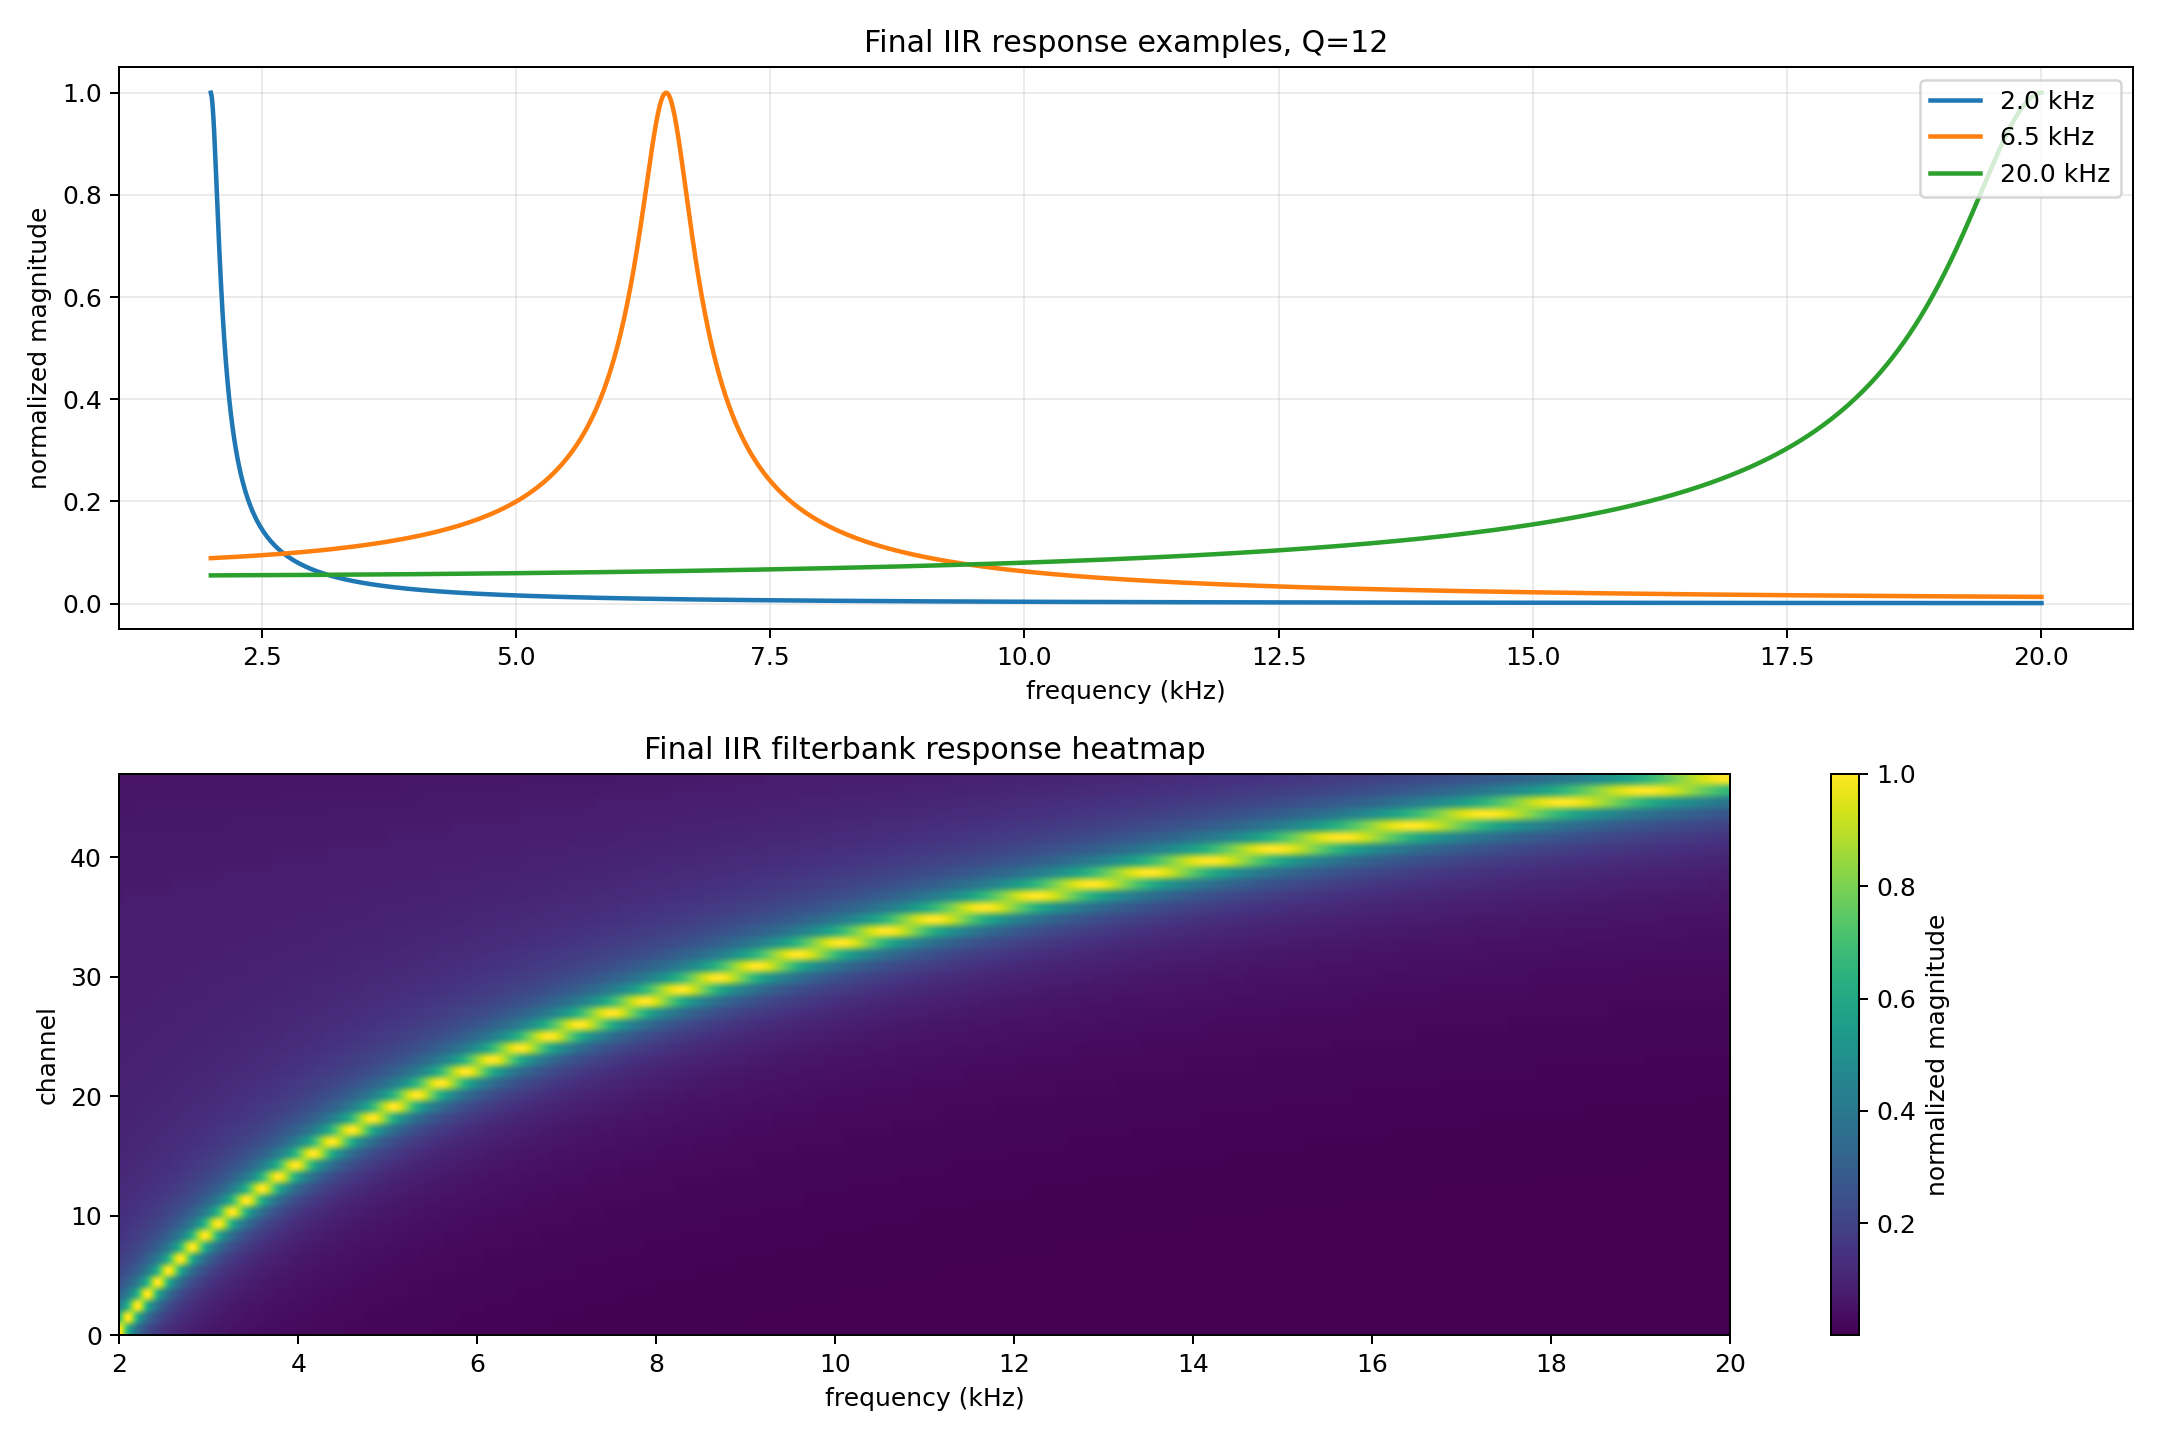
\includegraphics[height=5cm]{3_Modelling/cochlea/IIR_filterbank.png}
        \label{}
        \caption{}
    \end{subfigure}
    \hspace{0.1cm}
    % Panel B
    \begin{subfigure}[t]{0.45\textwidth}
        \textbf{\large B}\\[0.5ex]  % Forces the bold 'B' to the top left
        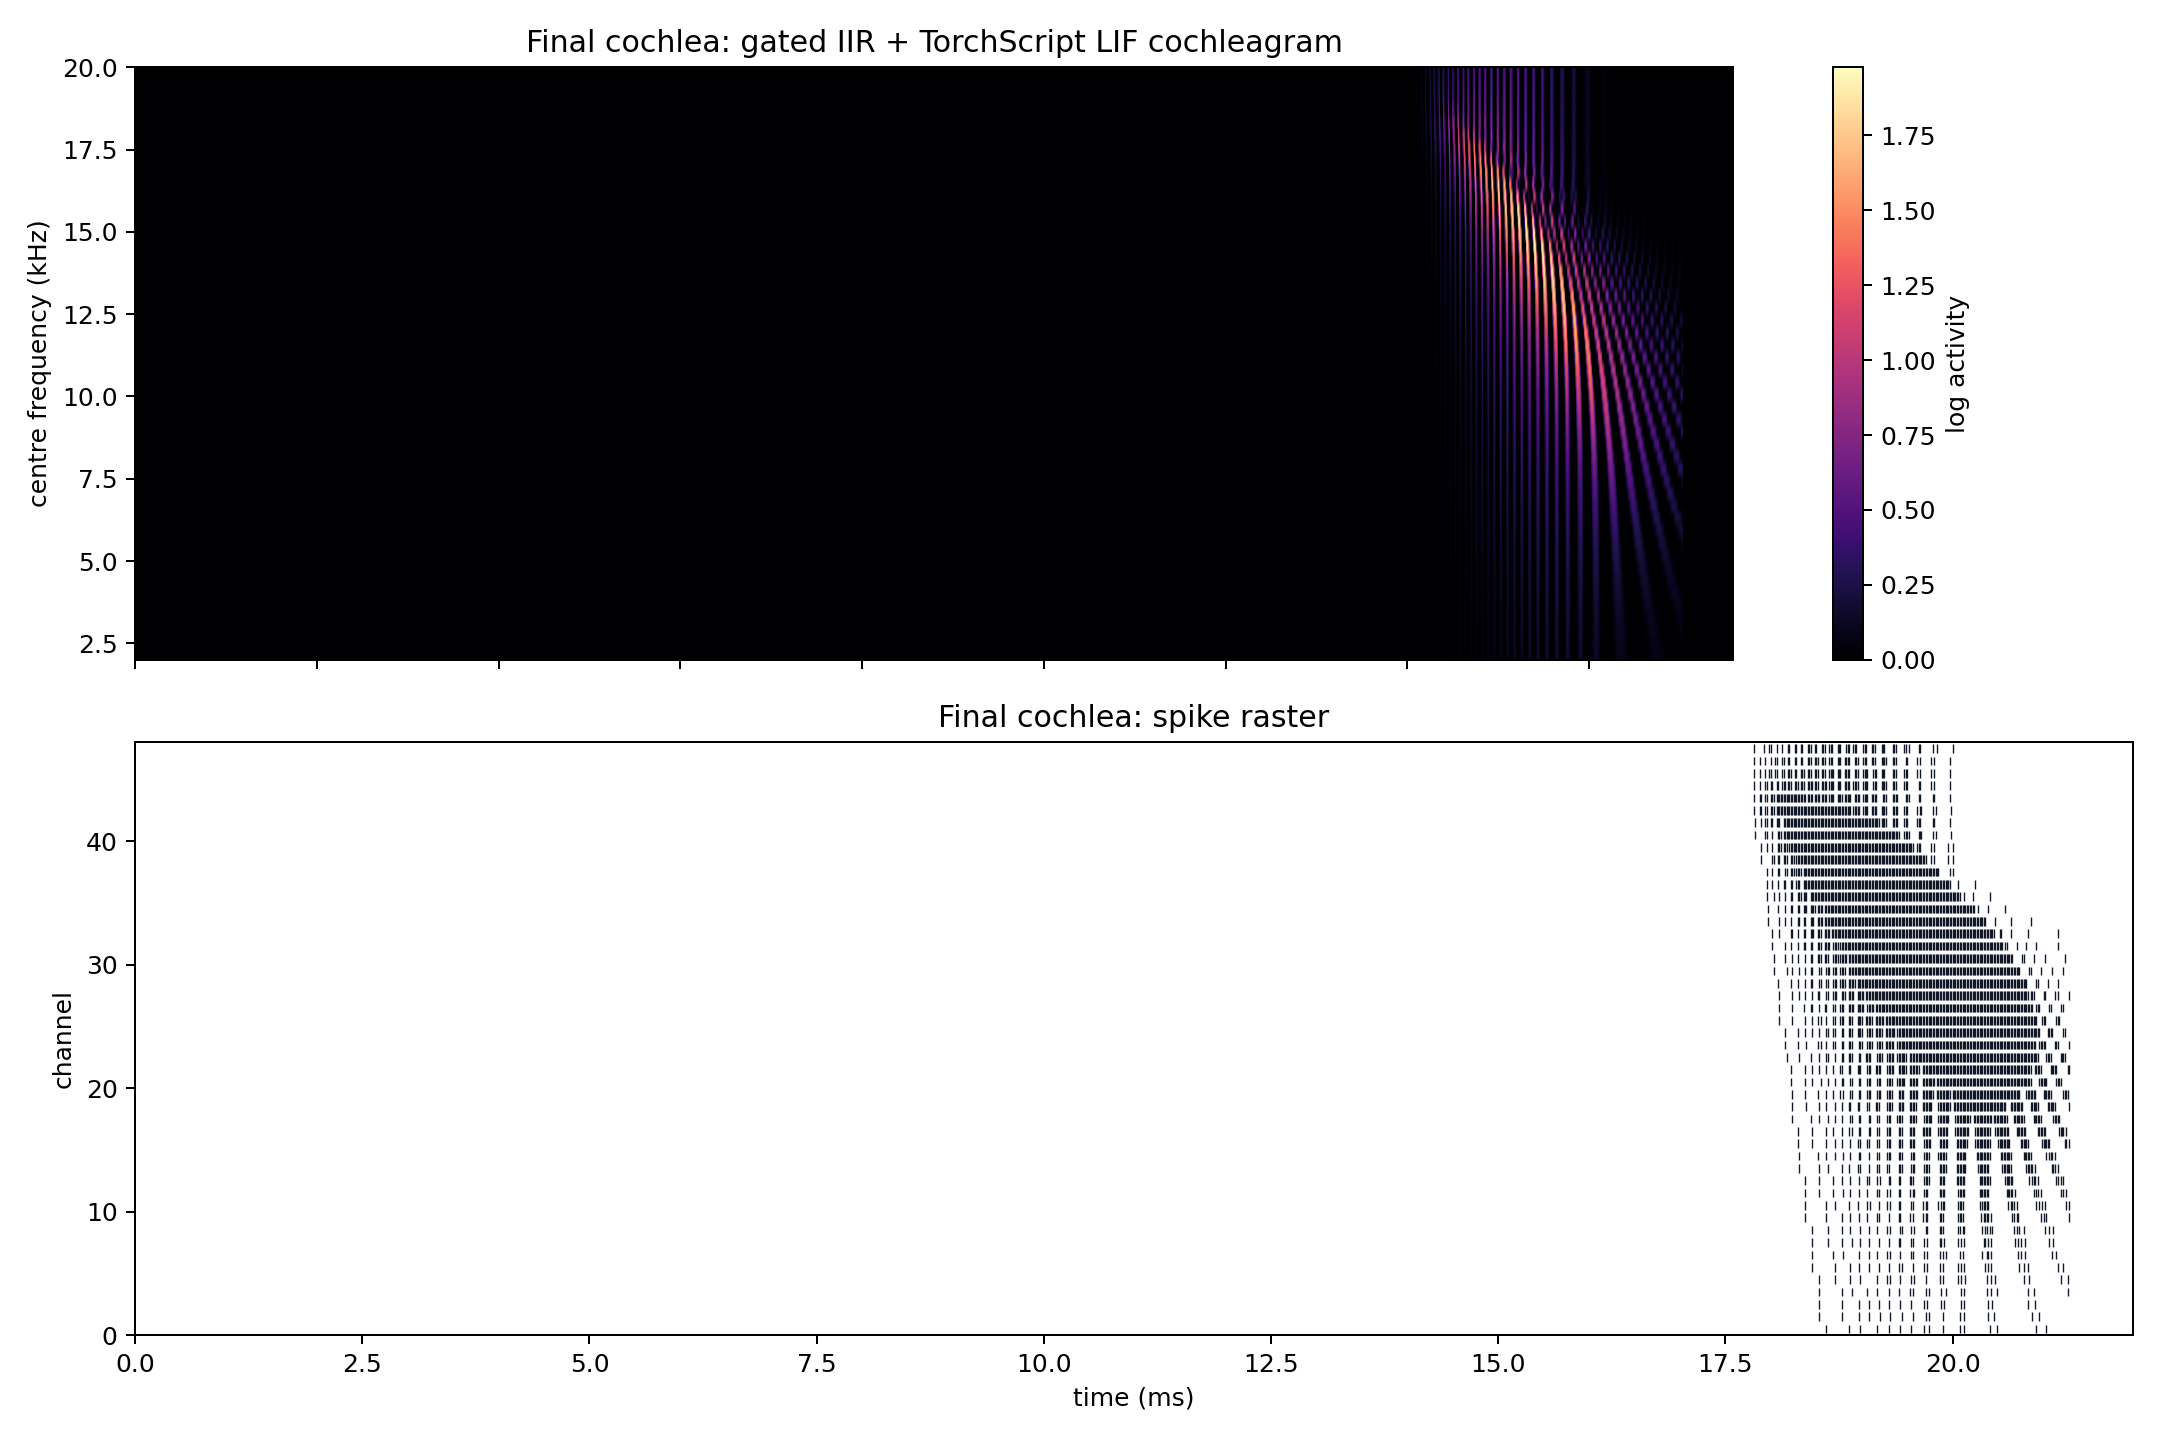
\includegraphics[height=5cm]{3_Modelling/cochlea/CSR.png}
        \caption{}
        \label{}
    \end{subfigure}

    \caption{A: IIR filterbank response. B: Cochleagram and cochlear spike raster (CSR)}
    \label{fig:cochlea_results}
\end{figure}

\subsection{Half-wave Rectification and LIF Encoding}

To transform the biphasic, zero-mean acoustic oscillations into a unipolar physiological driving current, the raw filter outputs undergo half-wave rectification. This non-linear step models the directional gating of inner hair cells, which only activate from amplitudes in one direction.:
\begin{equation}
    e_c[t] = \max\left(y_c[t], 0\right).
\end{equation}
This rectification prevents mutual cancellation of positive and negative signal phases during downstream temporal integration, and also models the biological constraint of only having positive excitatory neural signals.

The rectified receptor potential $e_c[t]$ serves as the continuous input current $I_c[t]$ to a layer of Leaky Integrate-and-Fire (LIF) spiking neurons. The sub-threshold membrane potential $v_c[t]$ accumulates charge according to a dynamic decay factor $\beta(t)$:
\begin{equation}
    v_c[t] = \beta(t)v_c[t-1] + e_c[t].
\end{equation}

When the membrane potential meets or exceeds a threshold $V_{th}$, the neuron discharges a binary spike event ($S_c[t] = 1$), otherwise, it remains quiescent ($S_c[t] = 0$):
\begin{equation}
    S_c[t] = \mathbb{I}\left[v_c[t] \geq V_{th}\right],
\end{equation}
where $\mathbb{I}[\cdot]$ is the indicator function. Following a spike event, a subtractive reset mechanism lowers the membrane voltage while imposing a strict lower bound at zero:
\begin{equation}
    v_c[t] \leftarrow \max\left(0, v_c[t] - S_c[t]\phi\right).
\end{equation}

Initially, a low-pass filter was used before the LIF spike encoding stage, but the low-pass nature of the LIF neuron does this implicitly.

\subsection{Neuronal IIR Filter through Mathematical Equivalence}

Whilst the cochlea itself is a mechanical system (rather than neuronal), an experiment was undertaken as to whether the IIR filters used could be replaced by a neuron-based system. This tested three setups: the Direct-Form IIR filter, an RF neuron acting as a resonant filter, and an excitatory-inhibitory (E/I) recurrence loop of neuron populations. We will analyse the RF neuron now in a state space form to account for the imaginary component of its voltages.

In the linear analog domain, the Direct-Form IIR filter, the State-Space RF neuron, and the E/I population loop are mathematically equivalent second-order resonators sharing identical poles, characteristic equations, and stability criteria. Further to this, the RF neuron and the E/I loop are two expressions of exactly the same equations, with the imaginary (or `quadrature') part of the RF neuron being equivalent to the inhibitory state of the E/I system.

The Direct-Form IIR filter tracks a single output scalar using historical, time-delayed output recurrences:
\begin{equation}
    y[n] = b_0 x[n] + 2p\cos(\phi)y[n-1] - p^2y[n-2]
\end{equation}

In contrast, the RF neuron and E/I circuit expose their internal dynamics via a two-dimensional state-space rotation matrix. Mapping the primary voltage/excitatory state to $v[n]$ (or $E[n]$) and the orthogonal quadrature/inhibitory state to $u[n]$ (or $I[n]$) yields the coupled system:
\begin{equation}
    \begin{bmatrix} v[n] \\ u[n] \end{bmatrix} = \begin{bmatrix} p\cos(\phi) & -p\sin(\phi) \\ p\sin(\phi) & p\cos(\phi) \end{bmatrix} \begin{bmatrix} v[n-1] \\ u[n-1] \end{bmatrix} + \begin{bmatrix} g \\ 0 \end{bmatrix} x[n]
\end{equation}

This idea for the E/I loop is shown in Figure \ref{fig:ei_population_resonator}.

\begin{figure}[htbp]
    \centering
    % Ensure you have \usepackage{tikz} and \usetikzlibrary{positioning, arrows.meta, calc} in your preamble
    \begin{tikzpicture}[
        >=Stealth,
        node distance=2cm and 2.5cm,
        font=\sffamily\small,
        % Define block styles
        block/.style={rectangle, draw, rounded corners, thick, minimum width=2.6cm, minimum height=1.5cm, align=center},
        E_node/.style={block, fill=blue!5, draw=blue!70!black},
        I_node/.style={block, fill=red!5, draw=red!70!black},
        io/.style={circle, draw, thick, fill=gray!5, minimum size=1.0cm, align=center},
        % Arrow styles
        line/.style={draw, thick, ->},
        inh_line/.style={draw, thick, ->, red!80!black}
    ]

        % --- Nodes ---
        \node[io] (in) {$x[n]$};
        
        \node[E_node, right=of in] (E) {
            \textbf{Excitatory (E)} \\ 
            Population State \\ 
            $E[n]$
        };
        
        \node[I_node, below=1.8cm of E] (I) {
            \textbf{Inhibitory (I)} \\ 
            Quadrature State \\ 
            $I[n]$
        };
        
        \node[io, right=of E] (out) {$O[n]$};

        % --- Main Feedforward Path ---
        \path[line] (in) -- node[above] {$g$} (E);
        \path[line] (E) -- node[above] {spikes} (out);
        
        % --- Coupling Loops (The Rotation Matrix) ---
        % Forward Excitation: E -> I
        \path[line] ($(E.south east)!0.3!(E.south)$) -- 
            node[right, pos=0.5] {$+r\sin(\phi)$} 
            ($(I.north east)!0.3!(I.north)$);
            
        % Delayed Negative Feedback: I -> E
        \path[inh_line] ($(I.north west)!0.3!(I.north)$) -- 
            node[left, pos=0.5] {$-p\sin(\phi)$} 
            ($(E.south west)!0.3!(E.south)$);
            
        % --- Self-Decay Loops (Damping terms) ---
        % E Self-loop
        \draw[line] ([xshift=+0.25cm]E.north) .. controls +(0.4, 0.8) and +(-0.4, 0.8) .. ([xshift=-0.25cm]E.north)
            node[above, midway] {$p\cos(\phi)$};
            
        % I Self-loop
        \draw[line] ([xshift=+0.25cm]I.south) .. controls +(0.4, -0.8) and +(-0.4, -0.8) .. ([xshift=-0.25cm]I.south)
            node[below, midway] {$p\cos(\phi)$};

    \end{tikzpicture}
    \caption{Architectural topology of the linear Excitatory/Inhibitory (E/I) population loop configured as a state-space resonator. The system implements a two-dimensional rotation matrix where self-decay properties are governed by $\cos(\phi)$ scaling, and orthogonal coupling is established via balanced phase-delayed feedback lines scaling by $\pm\sin(\phi)$. This network architecture maps an identical complex-conjugate pole profile to the direct-form second-order IIR filter template.}
    \label{fig:ei_population_resonator}
\end{figure}


Applying the $\mathcal{Z}$-transform reveals the underlying algebraic identity. The direct-form and state-space transfer functions are defined respectively as:
\begin{equation}
    H_{\text{direct}}(z) = \frac{b_0}{1 - 2r\cos(\theta)z^{-1} + r^2z^{-2}}
\end{equation}
\begin{equation}
    H_{\text{state}}(z) = \frac{g(1 - r\cos(\theta)z^{-1})}{1 - 2r\cos(\theta)z^{-1} + r^2z^{-2}}
\end{equation}

Because both implementations share an identical denominator polynomial, their resonant behavior is governed by the exact same complex-conjugate pole pairs:
\begin{equation}
    z = p e^{\pm j\phi}
\end{equation}
The difference between these is in the numerator, where the direct form has no zeros, while the state space form has a zero at $z=r\cos{\theta}$ which represents the single-timestep processing delay of the second state.  

This mathematical equivalence is strictly conditional upon the systems remaining entirely linear and continuous, and so does not account for the spiking dynamics very well. The introduction of any neuromorphic or biological non-linearities, including hard spiking thresholds, discontinuous state resets, refractory periods, asymmetric half-wave rectification, or finite synaptic propagation delays, violates the linear superposition principle. Once these event-driven mechanics are activated, the models diverge completely into independent, non-linear dynamical systems with distinct state trajectories and bifurcation characteristics.


\subsection{Noise and Dynamic Thresholding}

The initial threshold and decay rates of the LIF neurons in the cochlea model were initially set to arbitrary values. The threshold was set to a low value of 0.42 to get a clear, dense spiking response in the zero-noise environment. The decay rate $\beta$ was set to 0.88. This was sufficient for the zero-noise case, but then, as soon as noise was added, the low threshold and slow decay made the system fail immediately.

To fix this, various thresholds were tested, as shown in Figure \ref{fig:threshold_sweep}. Sweeps for $\beta$ were also done, with a smaller beta showing a less noisy CSR, but a less prominent desired signal, similar to increasing the threshold.

\begin{figure}[h]
    \centering
    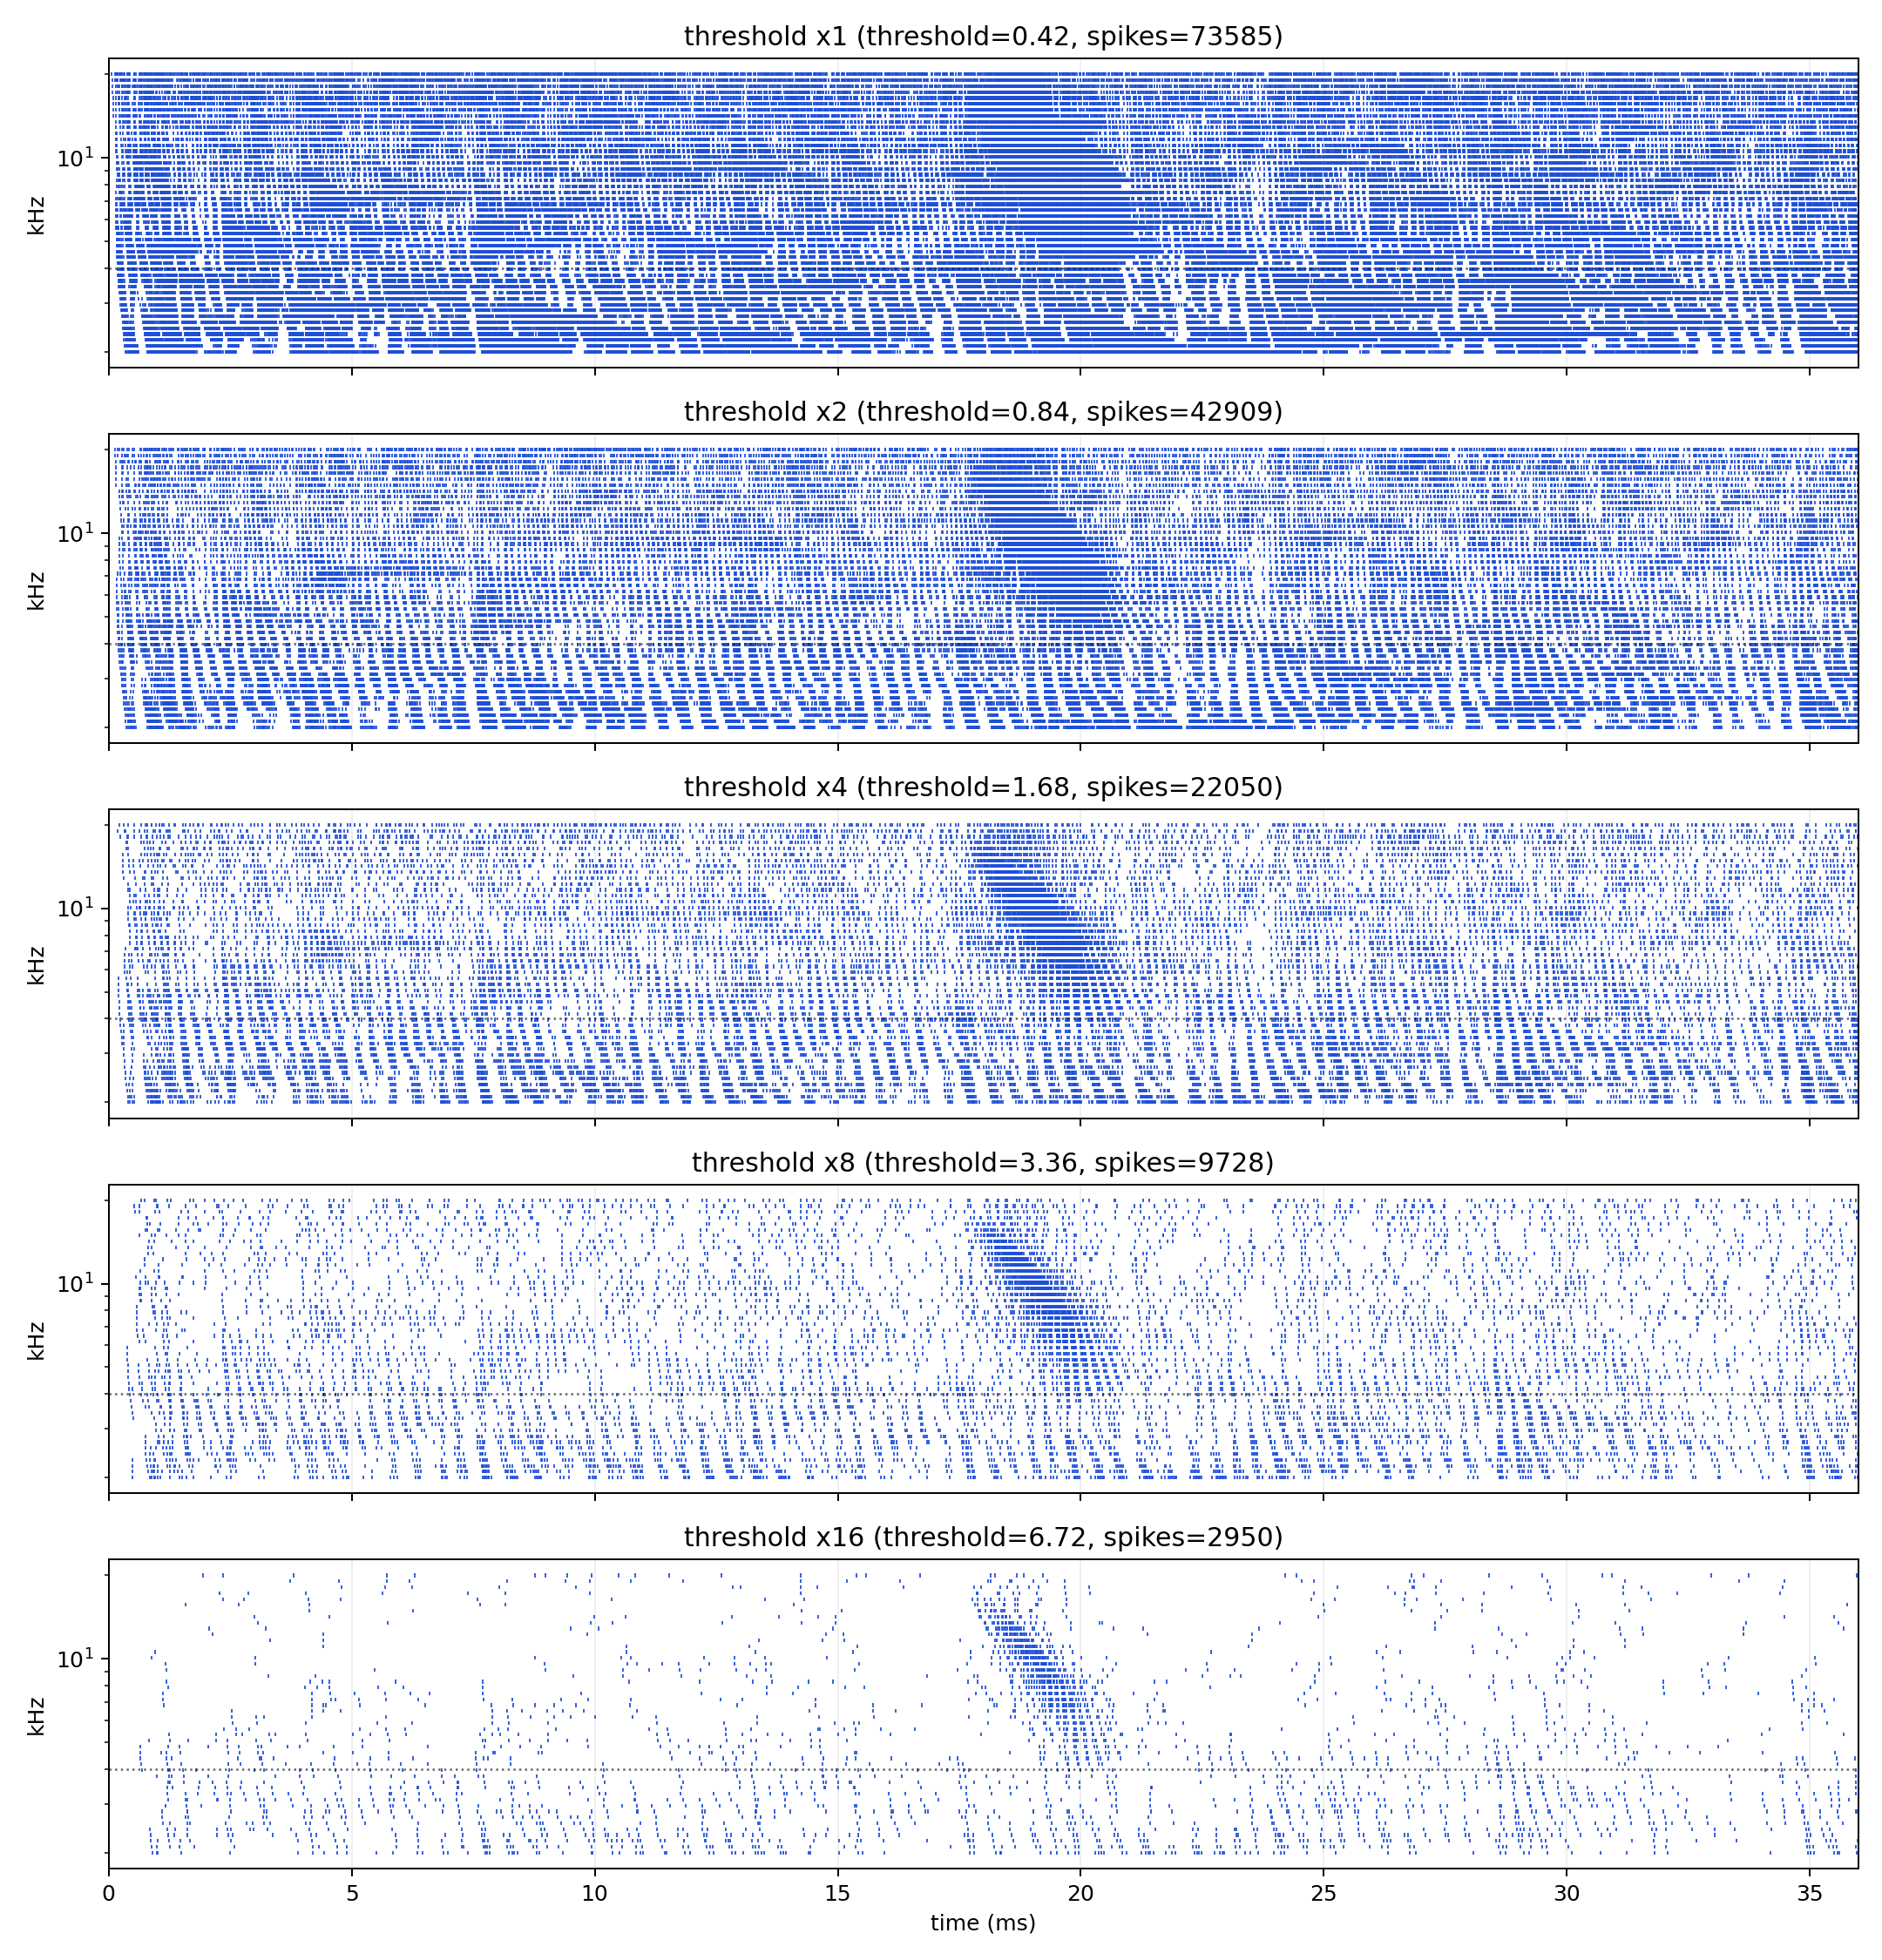
\includegraphics[width=1\textwidth]{3_Modelling/cochlea/threshold_sweep.png}
    \caption{LIF threshold tests for cochlear spike encoding at a test case of 3m.}
    \label{fig:threshold_sweep}
\end{figure}

From this testing, a threshold 16x the original value, i.e. $V_{th}=6.72$, and a decay value of $\beta = 0.5$ were selected by inspection of the CSRs. This had much better results, however for objects that were far away, the echo would be much weaker, and cause very few spikes to fire. This was solved by a dynamic threshold and dynamic decay rate, such that the longer the echo took to return, the lower the threshold and higher the decay rate, encouraging spiking without having noise trigger spikes too early. These followed the following schedules:

\begin{equation}
    V_{\text{th}}(t) = V_{\text{base}} \left( V_{\text{floor}} + (V_{\text{start}} - V_{\text{floor}}) e^{-\frac{t}{\tau_{\text{th}}}} \right)
\end{equation}
where $V_{\text{base}} = 0.42$, $V_{\text{start}} = 16$, $V_{\text{floor}} = 2.5$, and $\tau_{\text{th}} = 16\text{~ms}$.

\begin{equation}
    \beta(t) = \beta_{\text{start}} + (\beta_{\text{end}} - \beta_{\text{start}}) \left( 1 - e^{-\frac{t}{\tau_{\beta}}} \right)
\end{equation}
where $\beta_{\text{start}} = 0.20$, $\beta_{\text{end}} = 0.60$, and $\tau_{\beta} = 24\text{~ms}$.

An example of the effect of these dynamic schedules is shown in Figure \ref{fig:schedule}.

\begin{figure}[h]
    \centering
    
\includegraphics[width=1\textwidth]{3_Modelling/cochlea/schedule.png}
    \caption{Dynamic threshold and decay schedule example case at 5m compared to static cochlea. A line is shown at 4kHz, where all spikes below this level are not passed on.}
    \label{fig:schedule}
\end{figure}

The dynamic threshold and decay schedule can be interpreted as a simplification of several biological effects: hair-cell adaptation, cochlear nerve dynamic range, and most notably, the stapedius response of the voluntary middle ear muscle contractions in the bat. Rather than modelling each of these separately, the model uses a time-dependent excitability schedule that suppresses early noise and stabilises spike timing across target distances.

The tuning of this system was done in a manner to achieve functionality through inspection of the CSR, rather than numerical tuning. This is an example of how many of the systems have room to be optimised further through tuning, or possibly utilising targeted training of the system on key parameters. This process of manually hand-tuning and hand-designing the system highlights which of these key parameters should be focused on if full training of the system were ever to take place. 

\section{The Distance Pathway}

The distance pathway estimates range from the echo time-of-flight. It uses the emitted call as an internal reference (CD) and compares this reference with the received echo. The biological analogue is a population of delay-tuned FM-FM neurons that respond when the call-related input and echo-related input arrive at a preferred temporal separation, with a bend of supporting signals to improve this computation. Figure \ref{fig:distance_flowchart} shows the model developed, with each block representing a different computation on the spikes. These computations are modelled on the neurobiology of the bat, but are functionally simplified.


\begin{figure}[htbp]
    \centering
    \begin{tikzpicture}[
        block/.style={draw, rectangle, minimum height=1.2cm, minimum width=2.6cm, rounded corners=3pt, line width=0.8pt, align=center, fill=white, font=\small\sffamily\bfseries},
        nobox/.style={rectangle, minimum height=1.2cm, minimum width=2.6cm, align=center, font=\small\sffamily\bfseries},
        arrow/.style={-{Stealth[scale=1.2]}, line width=0.8pt}
    ]
    
    % Main Horizontal Chain
    \node (raster) [nobox, minimum width =1.5cm] {CSR};
    \node (vcn) [block, right=0.8cm of raster] {VCN/VNLL\\Model};
    \node (ic) [block, minimum width =1.5cm, right=1.5cm of vcn] {IC};
    \node (ac) [block, minimum width =1.5cm, right=0.8cm of ic] {AC};
    \node (sc) [block, minimum width =1.5cm, right=0.8cm of ac] {SC};
    \node (readout) [nobox, right=0.8cm of sc] {Distance\\Readout};
    
    % Detour Node (Below and slightly right of VCN)
    \node (dnll) [block, below=1.0cm of vcn, xshift=1.8cm] {3) DNLL};
    \node (cd) [block, minimum width =1.5cm, below=1.0cm of ac] {CD};
    
    % Connections
    \draw [arrow] (raster) -- (vcn);
    \draw [arrow] (vcn) -- (ic); % Direct feed
    
    % Detour Routing
    \draw [arrow] (vcn.south) |- (dnll.west);
    \draw [arrow, dashed] (dnll.east) -| ([xshift=-0.2cm]ic.south);
    \draw [arrow] (cd.west) -| ([xshift=+0.2cm]ic.south);
    
    
    % Remaining Chain
    \draw [arrow] (ic) -- (ac);
    \draw [arrow] (ac) -- (sc);
    \draw [arrow] (sc) -- (readout);
    
    \end{tikzpicture}
    \caption{Distance mapping pipeline featuring parallel brainstem inhibitory pathways.}
    \label{fig:distance_flowchart}
\end{figure}

\subsection{VCN/VNLL Onset Processing}

Downstream pathways require sharper timing than the raw cochlear spike raster provides. The VCN/VNLL stage is therefore simplified to an onset detector. A combined VCN/VNLL model was used to simplify the volume dependent latency of the VCN that is counteracted by the VNLL into a simple, constant (or adjusted) latency system. This model does not fix the latency of the cochlear LIF neurons, however. This task has been shifted to a correction in the CD signal, discussed in the next sub section.

In the VCN/VNLL model, a multi-channel consensus detector requires activity across neighbouring frequency channels before accepting an onset. This helps reject isolated noise spikes and creates a cleaner sweep-like onset representation. This was a simplified model of the endbulb of Held synapses and octopus cells, which have multiple connections to make them spike quickly when a broadband signal is received.

The biological VCN/VNLL system is more complex than this. In particular, real circuits include latency encoding, inhibitory timing compensation, and multiple parallel projections. The model replaces this with calibrated onset extraction because the goal is not to reproduce the full hindbrain circuit, but to deliver the computational object needed by the IC: a reliable estimate of when each frequency component of the echo arrived.

The VCN/VNLL onset consensus model has the following features:
\begin{itemize}
    \item Frequency mask boundary: $f_c \geq 4\text{~kHz}$
    \item Neighborhood channel radius: $\Delta c = \pm 2\text{~channels}$
    \item Neighborhood temporal radius: $\Delta t = \pm 8\text{~samples}$ ($\pm 125\text{~}\mu\text{s}$ at $64\text{~kHz}$)
    \item Density activation threshold: $\Theta_{\text{consensus}} = 3\text{~spikes}$
\end{itemize}

These are implemented as follows. Let $S_c[t] \in \{0,1\}$ represent the raw dynamic spike output from tonotopic channel $c$ at discrete time step $t$, and let $f_c$ denote the center frequency of that channel. 

First, a high-pass frequency mask isolates the ultrasonic echolocation band:
\begin{equation}
    R_c[t] = S_c[t] \cdot \mathbb{I}\left(f_c \geq 4\text{~kHz}\right),
\end{equation}
where $\mathbb{I}(\cdot)$ is the indicator function evaluating to 1 if the inner condition is satisfied, and 0 otherwise.

Next, a local consensus count $N_c[t]$ is evaluated by convolving a two-dimensional spatiotemporal window over the masked spike train:
\begin{equation}
    N_c[t] = \sum_{i=-2}^{2} \sum_{j=-8}^{8} R_{c+i}[t+j].
\end{equation}
This integration window spans a structural radius of $\pm 2$ tonotopic channels and a temporal window of $\pm 8$ sample bins. This system is essentially an approximated form of an LIF coincidence system.

A candidate VCN onset event, $C_c[t]$, is validated only if a local spike co-occurs with a dense neighborhood consensus:
\begin{equation}
    C_c[t] = R_c[t] \cdot \mathbb{I}\left(N_c[t] \geq \Theta_{\text{consensus}}\right),
\end{equation}
where $\Theta_{\text{consensus}} = 3$ represents the minimum required local spike density threshold.

Finally, to enforce a biological first-arrival onset rule and establish an absolute refractory period for the echo-ranging cycle, the finalized VCN output spike train $S_{\text{VCN}, c}[t]$ locks to the first validated candidate event per channel. 






\subsection{Corollary Discharge}

Because the system emits its own call, it has access to a corollary discharge (CD): an internal copy of the expected outgoing sweep. In the model, this is represented as a sweep of spikes across frequency channels. 

A cochlear latency vector is applied to the corollary discharge to account for the LIF neurons having volume-dependent latency behaviour. The frequency sweep is given by
\begin{equation}
    f(t) = f_{\text{start}} + (f_{\text{end}} - f_{\text{start}}) \frac{t}{T}
\end{equation}
and so the CD discharge time (i.e. the time after the call is emitted) for each channel is
\begin{equation}
    t_{\text{cd}, c} = T \cdot \frac{f_c - f_{\text{start}}}{f_{\text{end}} - f_{\text{start}}} + \ell_c
\end{equation}
where T is the duration of the sweep, and $\ell_c$ is the latency vector. This latency vector is measured empirically by testing the cochlea against the unadjusted CD and storing the differences as a vector.

For a target at distance $r$, the expected echo VCN onset for channel $c$ is then approximately:
\begin{equation}
t_{\text{echo},c}(r) = t_{\text{cd},c} + \frac{2r}{v_{\text{sound}}}
\end{equation}

This is what is tested in the IC coincidence detectors.

\subsection{DNLL Suppression}

The DNLL stage is modelled as a suppressive mechanism that reduces late or repeated echo responses after a primary onset has been detected. This is implemented using a delayed downstream inhibition to the IC. This is useful for a single-target localisation model because it prevents later noise or secondary reflections from dominating the distance map. The tradeoff is that this simple suppression would make multi-object tracking difficult. In biological terms, this is a plausible attentional or clutter-rejection mechanism, but in engineering terms, it is a single-object assumption. If multiple object detection was desired, this could be altered from a permanent inhibition to a decaying inhibition (this is also biologically grounded in the workings of the DNLL).

\subsection{IC Coincidence Detection}

The inferior-colliculus stage was modelled as a bank (i.e. a set) of distance-tuned coincidence detectors. Each candidate distance $r_k$ corresponds to a candidate acoustic round-trip delay
\begin{equation}
    \Delta_k = \frac{2r_k}{v_{sound}},
\end{equation}
For each frequency channel $c$, the model compares the VCN echo onset time $t_{\mathrm{echo},c}$ with the delayed corollary-discharge expectation
\begin{equation}
    t_{\mathrm{ref},c,k} = t_{\mathrm{cd},c} + \Delta_k .
\end{equation}

\subsubsection{Full LIF Delay-Line Formulation}

A more literal implementation would simulate a separate LIF coincidence neuron for every frequency channel $c$ and candidate delay $k$. This neuron would receive one input from the VCN echo onset and one input from the corollary-discharge template delayed by $\Delta_k$:
\begin{equation}
    v_{c,k}[n+1]
    =
    \beta_{\mathrm{IC}} v_{c,k}[n]
    +
    S_{\mathrm{echo},c}[n]
    +
    S_{\mathrm{cd},c}[n-\Delta_k],
\end{equation}
where $S_{\mathrm{echo},c}[n]$ is the VCN echo spike raster, $S_{\mathrm{cd},c}[n-\Delta_k]$ is the delayed corollary-discharge spike, and $\beta_{\mathrm{IC}}$ is the IC membrane retention factor. The output spike would be
\begin{equation}
    S_{\mathrm{IC},c,k}[n]
    =
    \mathbb{I}
    \left[
        v_{c,k}[n] \geq V_{\mathrm{th,IC}}
    \right],
\end{equation}
with subtractive reset
\begin{equation}
    v_{c,k}[n]
    \leftarrow
    v_{c,k}[n]
    -
    V_{\mathrm{th,IC}} S_{\mathrm{IC},c,k}[n].
\end{equation}
The population response for candidate distance $k$ would then be obtained by summing across frequency channels and time:
\begin{equation}
    I_k
    =
    \sum_c \sum_n S_{\mathrm{IC},c,k}[n].
\end{equation}

This is the most direct spiking interpretation: each distance bin is represented by a set of delay-line LIF neurons, and a distance is favoured when echo and corollary-discharge spikes arrive close enough in time to exceed threshold.

\subsubsection{Closed-Form Coincidence Surrogate Used}

In the implemented model, the full LIF bank was replaced by a closed-form surrogate. This was possible because each channel contributes at most one relevant VCN onset spike and one corollary-discharge spike for a given candidate distance. For two unit input spikes separated by
\begin{equation}
    \delta_{c,k}
    =
    \left|
        t_{\mathrm{echo},c}
        -
        \left(
            t_{\mathrm{cd},c}
            +
            \Delta_k
        \right)
    \right|,
\end{equation}
the peak membrane potential of a leaky integrator is
\begin{equation}
    m_{c,k}
    =
    1
    +
    \beta_{\mathrm{IC}}^{\delta_{c,k}}.
\end{equation}
If the spikes are simultaneous, $\delta_{c,k}=0$ and $m_{c,k}=2$. If they are separated in time, the first spike decays before the second arrives, reducing the peak response.

The channel contribution is then thresholded using a rectified response:
\begin{equation}
    s_{c,k}
    =
    \left[
        m_{c,k}
        -
        V_{\mathrm{th,IC}}
    \right]_+,
\end{equation}
where $[x]_+=\max(x,0)$. The raw IC distance population is
\begin{equation}
    I_k^{\mathrm{raw}}
    =
    \sum_c s_{c,k}.
\end{equation}

This produces the same peak-response logic as a two-spike LIF coincidence detector, but avoids explicitly simulating every membrane voltage over every time step, hugely speeding up simulation times.

\subsubsection{Sweep Facilitation}

The final IC model also includes a soft facilitation term in order to improve noise robustness internally. This was done to lay the foundation for a more complex system that may not guarantee one spike per channel (e.g. for multiple object localisation). The FM call should produce a consistent sweep across neighbouring frequency channels, so a candidate distance is more reliable if adjacent channels support a similar delay. For each channel and candidate distance, a local sweep-consistency term $F_{c,k}$ is computed from neighbouring channels:
\begin{equation}
    F_{c,k}
    =
    \frac{1}{|\mathcal{N}(c)|}
    \sum_{j \in \mathcal{N}(c)}
    \exp
    \left(
        -
        \frac{
            \left|
                t_{\mathrm{echo},j}
                -
                \left(
                    t_{\mathrm{cd},j}
                    +
                    \Delta_k
                \right)
            \right|
        }{
            \tau_{\mathrm{facil}}
        }
    \right),
\end{equation}
where $\mathcal{N}(c)$ is the set of neighbouring frequency channels and $\tau_{\mathrm{facil}}$ controls the tolerance of the facilitation.

The facilitated IC response is then
\begin{equation}
    I_k
    =
    \sum_c
    s_{c,k}
    \left(
        1
        +
        g_{\mathrm{facil}}F_{c,k}
    \right),
\end{equation}
where $g_{\mathrm{facil}}$ is the facilitation gain.

This term is not itself a LIF mechanism. It is a higher-level IC abstraction that softly boosts distance hypotheses supported by a coherent FM sweep, rather than treating each frequency channel as an independent coincidence measurement. This was chosen over a cascading gating mechanism so that there is not a high dependence on the first few high frequencies of the sweep, and instead encourages responses measured from sweeping inputs.

\subsection{AC Sharpening}

The raw IC population is passed through an AC-like topographic sharpening stage. This collapses the IC readout across the frequency channels to get distance estimations, then uses a Mexican-hat sharpening profile: local excitation around a candidate distance and broader inhibition around its neighbours. In simplified form:
\begin{equation}
    A = K_{\text{MH}} C,
\end{equation}
where $C$ is the IC candidate population and $K_{\text{MH}}$ is the Mexican-hat kernel. This sharpens the distance peak while retaining a smooth population code. Figure \ref{fig:AC_MH} visualises the kernel. 

\begin{figure}[h]
    \centering
    
\includegraphics[width=1\textwidth]{3_Modelling/distance/AC_MH.png}
    \caption{AC Mexican Hat kernel}
    \label{fig:AC_MH}
\end{figure}

A narrow excitatory Gaussian and broader inhibitory Gaussian define the lateral interaction kernel:
\begin{equation}
K = G_{\sigma_{\mathrm{exc}}} - g_{\mathrm{inh}}G_{\sigma_{\mathrm{inh}}}
\end{equation}
where $G_{\sigma}$ represents a zero-mean discrete Gaussian distribution with variance $\sigma^2$, where the distribution variable is the distance-bin offset.

This kernel is convolved with the IC distance population and added back to the original IC activity before rectification:
\begin{equation}
    A = \left[I + K * I\right]_+
\end{equation}
The residual term preserves the original delay evidence, while the Mexican-hat term sharpens local peaks and suppresses broad neighbouring activity. After tuning the parameters selected for this were: $\sigma_{exc} = 2$ bins, $\sigma_{inh} = 8$ bins, and $g_{inh} = 0.58$, where a bin is a distance grid step.

Whilst the AC is biologically home to FM-FM neurons as well, the simplification was made to use one set of delay-tuned FM-FM neurons and coincidence detectors. These were put in the IC block to reflect the raw arithmetic nature of the IC, and then the AC organises and sharpens these signals into distance readout signals, which are then passed onto the SC to decode.

\subsection{SC Distance Readout}

The SC was modelled for all three pathways as the measurement readout system. To start, all three pathways used a simple readout SC model.

Once the AC neural population code has been sent to the SC, a direct centre-of-mass (COM) readout can decode distance from this population:
\begin{equation}
    \hat{r} = \frac{\sum_k A_k r_k}{\sum_k A_k}.
\end{equation}
The final SC model instead passes the AC population into an SC line attractor model before decoding. This continuous attractor neural network model (CANN) readout will be discussed later.

\section{The Azimuth Pathway}

The azimuth pathway estimates horizontal angle from binaural differences. The model used the two primary pathways for utilising ITD and ILD, however, we simplified these two to be frequency independent, due to the frequency-independent head shadow. Due to this, both ITD and ILD can be used at any frequency, so we tested which was more accurate. The overall system for both pathways is shown in Figure \ref{fig:azimuth_flowchart}. It should be noted that the two main pathways have different VCN models.


\begin{figure}[htbp]
    \centering
    \begin{tikzpicture}[
        block/.style={draw, rectangle, minimum height=1.1cm, minimum width=2.5cm, rounded corners=3pt, line width=0.8pt, align=center, fill=white, font=\small\sffamily\bfseries},
        nobox/.style={rectangle, minimum height=1.1cm, minimum width=2.5cm, align=center, font=\small\sffamily\bfseries},
        arrow/.style={-{Stealth[scale=1.2]}, line width=0.8pt}
    ]
    
    % --- TOP ROW: LEFT PATHWAY ---
    \node (l_raster) [nobox] {Left CSR};
    \node (l_vcn) [block, right=0.8cm of l_raster] {Left VCN};
    \node (l_mntb) [block, below=0.3cm of l_vcn, xshift=2.5cm] {Left MNTB};
    \node (l_lso) [block, right=3cm of l_vcn] {Left LSO};
    
    % --- BOTTOM ROW: RIGHT PATHWAY ---
    \node (r_raster) [nobox, below=4.4cm of l_raster] {Right CSR};
    \node (r_vcn) [block, right=0.8cm of r_raster] {Right VCN};
    \node (r_mntb) [block, above=0.3cm of r_vcn, xshift=2.5cm] {Right MNTB};
    \node (r_lso) [block, right=3cm of r_vcn] {Right LSO};
    
    % --- MIDDLE ROW: CONVERGENCE ZONE ---
    \node (mso) [block, below=1.65cm of l_vcn, xshift=-1.5cm] {Combined\\MSO};
    \node (ic) [block, below=1.65cm of l_lso, minimum width=1.5cm] {IC};
    \node (sc) [block, right=0.8cm of ic, minimum width=1.5cm] {SC};
    \node (readout) [nobox, right=0.8cm of sc] {Azimuth\\Readout};
    
    % --- ARROWS ---
    
    % Ipsilateral Connections
    \draw [arrow] (l_raster) -- (l_vcn);
    \draw [arrow] (r_raster) -- (r_vcn);
    \draw [arrow] (l_vcn) -- (l_lso.west);
    \draw [arrow] (r_vcn) -- (r_lso.west);
    
    % Cross-talk (Contralateral MNTB Inhibitions)
    \draw [arrow] (l_vcn.south) -- ([yshift=0.5cm]r_mntb.west);
    \draw [arrow] (r_vcn.north) -- ([yshift=-0.5cm]l_mntb.west);
    \draw [arrow, dashed] (l_mntb) -- (l_lso);
    \draw [arrow, dashed] (r_mntb) -- (r_lso);
    
    % MSO Bilateral Feed
    \draw [arrow] ([xshift=-0.2cm]l_vcn.south) -- (mso.north);
    \draw [arrow] ([xshift=-0.2cm]r_vcn.north) -- (mso.south);
    
    % Unification into Midbrain Network
    \draw [arrow] (l_lso.south) -- (ic.north);
    \draw [arrow] (mso) -- (ic);
    \draw [arrow] (r_lso.north) -- (ic.south);
    
    % Output Track
    \draw [arrow] (ic) -- (sc);
    \draw [arrow] (sc) -- (readout);
    
    \end{tikzpicture}
    \caption{Binaural Azimuth processing network showing MSO time-delay pathway for ITD and cross-contralateral LSO/MNTB pathway for ILD.}
    \label{fig:azimuth_flowchart}
\end{figure}

\subsection{MSO ITD Pathway}

The ITD branch uses separate-ear VCN onset rasters. Each ear is passed through the dynamic cochlear spike encoder and then through the same VCN consensus onset detector used in the distance pathway. This produces one accepted onset time per frequency channel where reliable left and right activity is present. These are then fed into a Jeffress-style coincidence detection system in the model for a combined MSO, as shown in Figure \ref{fig:jeffress_mso_model}. The response of this system is then passed onto the IC.


\begin{figure}[htbp]
    \centering
    \begin{tikzpicture}[
        >=Stealth,
        font=\sffamily\small,
        line width=1.0pt,
        % --- Node Styles ---
        vcnNode/.style={rectangle, draw=gray!70, fill=gray!5, thick, rounded corners=3pt, minimum width=2.0cm, minimum height=0.9cm, font=\small\sffamily\bfseries},
        msoNode/.style={circle, draw=purple!70!black, fill=purple!5, thick, minimum size=1.0cm, align=center, font=\scriptsize\sffamily\bfseries},
        % --- Connection Styles ---
        leftLine/.style={->, draw=teal!80!black, line width=1.2pt},
        rightLine/.style={->, draw=orange!80!black, line width=1.2pt},
        dropLine/.style={->, line width=1.0pt, dashed, gray!70}
    ]

    % --- INPUT STATIONS (VCN) ---
    \node (LVCN) [vcnNode, text=teal!80!black] at (-1.5, 2.0) {Left VCN};
    \node (RVCN) [vcnNode, text=orange!80!black] at (7.5, 2.0) {Right VCN};

    % --- COINCIDENCE DETECTOR ARRAY (MSO) ---
    \node (mso1) [msoNode] at (0.5, 0.0) {MSO$_1$};
    \node (mso2) [msoNode] at (1.8, 0.0) {MSO$_2$};
    \node (mso3) [msoNode] at (3.0, 0.0) {MSO$_3$}; % Center
    \node (mso4) [msoNode] at (4.2, 0.0) {MSO$_4$};
    \node (mso5) [msoNode] at (5.5, 0.0) {MSO$_5$};

    \node[left=0.1cm of mso1, font=\small\sffamily\bfseries, text=purple!80!black, align=right] {Coincidence\\Detectors};

    % --- LEFT AXON DELAY LINE (Teal, sweeps Left-to-Right) ---
    % Main conduit line across the top
    \draw [leftLine] (LVCN.south) -- ++(0, -0.5) coordinate (Lstart) -- (5.5, 1) 
        node[midway, above, font=\scriptsize\sffamily\bfseries, text=teal!80!black] {Left Axonal Delay Line ($\tau_{\text{L}}$)};
    
    % Dropping collaterals into MSO nodes
    \draw [dropLine, teal!80!black] (0.5, 1) -- (mso1.north);
    \draw [dropLine, teal!80!black] (1.8, 1) -- (mso2.north);
    \draw [dropLine, teal!80!black] (3.0, 1) -- (mso3.north);
    \draw [dropLine, teal!80!black] (4.2, 1) -- (mso4.north);
    \draw [dropLine, teal!80!black] (5.5, 1) -- (mso5.north);

    % --- RIGHT AXON DELAY LINE (Orange, sweeps Right-to-Left) ---
    % Main conduit line across the bottom
    \draw [rightLine] (RVCN.south) -- ++(0, -2.55) coordinate (Rstart) -- (0.5, -1)
        node[midway, below, font=\scriptsize\sffamily\bfseries, text=orange!80!black] {Right Axonal Delay Line ($\tau_{\text{R}}$)};

    % Dropping collaterals into MSO nodes
    \draw [dropLine, orange!80!black] (5.5, -1) -- (mso5.south);
    \draw [dropLine, orange!80!black] (4.2, -1) -- (mso4.south);
    \draw [dropLine, orange!80!black] (3.0, -1) -- (mso3.south);
    \draw [dropLine, orange!80!black] (1.8, -1) -- (mso2.south);
    \draw [dropLine, orange!80!black] (0.5, -1) -- (mso1.south);

    % --- VISUAL GRADIENT KEYS / ANNOTATIONS ---
    \draw [->, line width=0.6pt, gray] (0, 1.6) -- node[above, font=\tiny\sffamily] {Increasing Delay} (3, 1.6);
    \draw [->, line width=0.6pt, gray] (6.5, -1.7) -- node[below, font=\tiny\sffamily] {Increasing Delay} (3.5, -1.7);
    
    \node [right=-0.4cm of mso5, font=\tiny\sffamily, text=teal!80!black, align=left, yshift=0.9cm] {Max Delay\\(Left Input)};
    \node [left=-0.4cm of mso1, font=\tiny\sffamily, text=orange!80!black, align=right, yshift=-0.9cm] {Max Delay\\(Right Input)};

    \end{tikzpicture}
    \caption{The Jeffress anatomical delay-line model implemented within the Medial Superior Olive (MSO) sub-circuit. Contralateral and ipsilateral inputs project antiparallel axonal branches across an array of coincidence-detecting principal cells. A given MSO neuron fires maximally when the physical interaural time difference (ITD) of an incoming echo wavefront is perfectly compensated for by the structural path length delay ($\Delta\tau = \tau_{\text{L}} - \tau_{\text{R}}$) of the matching collaterals.}
    \label{fig:jeffress_mso_model}
\end{figure}


For candidate azimuth $\theta_k$, the expected right-minus-left ITD is approximated by the far-field expression
\begin{equation}
    \Delta t_k = -\frac{d_{\mathrm{ear}}\sin\theta_k}{v_{sound}},
\end{equation}
where $d_{\mathrm{ear}}$ is the interaural spacing. In samples,
\begin{equation}
    \Delta n_k = f_s \Delta t_k .
\end{equation}

For each frequency channel $c$, the observed right-minus-left onset difference is
\begin{equation}
    \Delta n_c = n_{R,c} - n_{L,c}.
\end{equation}
A Jeffress-style coincidence detector scores how closely this observed ITD matches each candidate delay. Using the same two-spike LIF peak approximation as the distance pathway,
\begin{equation}
    m_{c,k}
    =
    1 + \beta_{\mathrm{ITD}}^{|\Delta n_c-\Delta n_k|},
\end{equation}
\begin{equation}
    a_{c,k}
    =
    \left[
        m_{c,k}
        -
        \vartheta_{\mathrm{ITD}}
    \right]_+ .
\end{equation}
where $m_{c,k}$ is the peak membrane response of the ITD coincidence detector for frequency channel $c$ and azimuth candidate $\theta_k$, $\beta_{\mathrm{ITD}}$ is the membrane retention factor of the ITD coincidence neuron, $\Delta n_c$ is the observed right-minus-left onset difference in samples for channel $c$, and $\Delta n_k$ is the expected right-minus-left delay in samples for candidate azimuth $\theta_k$.

The term $\vartheta_{\mathrm{ITD}}$ is the coincidence threshold, and $[\cdot]_+$ denotes rectification, $[x]_+=\max(x,0)$. Thus $a_{c,k}$ is the thresholded channel-level evidence that channel $c$ supports azimuth candidate $\theta_k$. The full ITD population $A_{\mathrm{ITD}}(\theta_k)$ is then obtained by summing this evidence over all valid frequency channels:
\begin{equation}
    A_{\mathrm{ITD}}(\theta_k)
    =
    \sum_c a_{c,k}.
\end{equation}
This is a simplified Jeffress-style model. It captures the essential idea of coincidence across ears, but does not model the full MSO/brainstem microcircuit. It also inherits a physical limitation: for small heads, ITDs are extremely small, so wide-angle or noisy conditions can make timing ambiguous. The acoustic simulator computes the two ear path lengths explicitly, but the candidate ITD grid uses a far-field sine approximation rather than a full spherical-head model.

It should also be noted that whilst the Jeffress-style MSO is a clear and logical model, there is evidence that it may be outdated, and an updated model involves balancing excitory and inhibitory responses, including the MNTB and the Lateral Nucleus of the Trapezoid Body (LNTB) in the pathway. This works similarly to the ILD pathway, but instead balances precise timing differences rather than level differences. The advantage of this system is increasing sensitivity around the $0 \degree$ line, however, the Jeffress style model was chosen for its simplicity and robustness to sub-optimal tuning.


\subsection{LSO/MNTB ILD Pathway}

The ILD branch estimates azimuth from left/right intensity imbalance. Unlike the ITD branch, it does not preserve precise onset timing. Instead, each ear is converted into a multi-threshold level code, as a functional model for the VCN for this sub-pathway, as well as integrating some of the behaviour of the cochlea.

For each frequency channel, the cochlear spike count is compared against a bank of varying thresholds. Louder inputs cross more thresholds and therefore produce a larger level code:
\begin{equation}
    X_L(c) =
    \sum_q
    \mathbb{I}
    \left[
        N_L(c) \geq \rho_q N_{\max}(c)
    \right],
\end{equation}
\begin{equation}
    X_R(c) =
    \sum_q
    \mathbb{I}
    \left[
        N_R(c) \geq \rho_q N_{\max}(c)
    \right],
\end{equation}
where $N_L(c)$ and $N_R(c)$ are the left and right cochlear spike counts in channel $c$, $\rho_q$ are the threshold fractions, and $N_{\max}(c)=\max(N_L(c),N_R(c),1)$ normalises the thresholds per channel. This normalisation has the trade-off of being less sensitive to distance/global loudness, but losing the absolute information about the volume of the signal. This was done as we are concerned with the relative binaural differences, rather than the absolute levels. 

This thresholding model is effectively an approximation for a bank of leaky-integrate neurons with no decay. This means the spikes across the entire time series are being counted up. An improved model would likely have a non-zero decay rate, which would allow for continuous measurement of the ILD and possible functionality for multi-object detection. This project simplified the model for a single pulse functionality.

LSO/MNTB systems were modelled as a comparison, represented as same-side excitation opposed by opposite-side inhibition:
\begin{equation}
    L_{\mathrm{left}}(c)
    =
    \left[
        w_E X_L(c)
        -
        w_I X_R(c)
    \right]_+,
\end{equation}
\begin{equation}
    L_{\mathrm{right}}(c)
    =
    \left[
        w_E X_R(c)
        -
        w_I X_L(c)
    \right]_+.
\end{equation}
This captures the functional role of the LSO/MNTB circuit: the LSO receives excitatory input from the ipsilateral (same side) ear and inhibitory input driven by the contralateral (opposite side) ear through the MNTB. The MNTB in reality receives an excitory signal and converts this into an inhibitory signal. This is simply modelled as a negative synaptic inhibitory weight $w_I$, which is set to 0.72 from tuning. The excitatory weight $w_E =1$. The reduced inhibitory weight allows the system to still have excitatory drive at $0\degree$ azimuth. These weights are another example of something that was tuned in the bottom-up design of the model, but could be marked as key variables for a future fully trainable model.

The ouputs of both LSOs are combined within the IC, where the final balancing comparison occurs. The resulting left-right opponent balance is
\begin{equation}
    b
    =
    \frac{
        \sum_c L_{\mathrm{right}}(c)
        -
        \sum_c L_{\mathrm{left}}(c)
    }{
        \sum_c L_{\mathrm{right}}(c)
        +
        \sum_c L_{\mathrm{left}}(c)
        +
        \epsilon
    }.
\end{equation}
Candidate azimuths are then scored by comparing this balance to the expected monotonic azimuth coordinate:
\begin{equation}
    A_{\mathrm{ILD}}(\theta_k)
    =
    D
    \exp
    \left[
        -
        \frac{
            \left(
                b-\sin\theta_k
            \right)^2
        }{
            2\sigma_{\mathrm{ILD}}^2
        }
    \right],
\end{equation}
where $D=\sum_c L_{\mathrm{left}}(c)+\sum_c L_{\mathrm{right}}(c)$ is the total opponent drive, reintegrating the absolute level information we lost in the normalisation process, to supply a confidence level such that signal responses give more confident information than noise readings.

\subsection{SC Readout}

The azimuth pathway produces a one-dimensional population code over candidate azimuths $\theta_k$. In the simplest readout, this population is decoded using a COM estimate, just like used in the distance pathway:
\begin{equation}
    \hat{\theta}
    =
    \frac{
        \sum_k A(\theta_k)\theta_k
    }{
        \sum_k A(\theta_k) + \epsilon
    },
\end{equation}
where $A(\theta_k)$ is the activity of the azimuth population at candidate angle $\theta_k$, and $\epsilon$ prevents division by zero.

This readout uses the whole population rather than only the maximum-activity bin. It therefore allows sub-bin estimates when activity is spread smoothly across neighbouring azimuth candidates. 

Initially, a weighted balance of the readouts from the ILD and ITD sub-pathways was used, however this would cause a full weighting on the most accurate pathway. This is discussed further in Chapter \ref{ch:results}. In reality, the brain uses ILD and ITD when they are most accurate, as per the duplex theory discussed in Chapter \ref{ch:background} (ITD at low frequencies, ILD at high frequencies). In our model, both can supply useful information for different cues and setups, but combining when to use which is not a simple task. We will explore this in the improved combined fusion readout.

\section{The Elevation Pathway}

The elevation pathway estimates vertical angle from monaural spectral shaping. Unlike distance and azimuth, elevation is not primarily a timing problem. It depends on how the pinna-like filter changes the frequency content of the echo. This naturally opens it up for higher errors, which is also seen in nature with bats. This is solved in nature by the fact that bats, and humans, both can move. Mammals often have reflexes to look in the direction of sounds, which can then utilise the more accurate systems. In our model, we often consider a perfect environment and known handcrafted conditions, so this may differ from the reality.

Figure \ref{fig:elevation_flowchart} shows the overall process. This is much simpler than the other pathways, as we have simplified the biology to a functional model of notch detection rather than full spectral inference. This means elevation is mostly estimated by computations within the DCN.

\begin{figure}[htbp]
    \centering
    \begin{tikzpicture}[
        block/.style={draw, rectangle, minimum height=1.2cm, minimum width=2.6cm, rounded corners=3pt, line width=0.8pt, align=center, fill=white, font=\small\sffamily\bfseries},
        nobox/.style={rectangle, minimum height=1.2cm, minimum width=2.6cm, align=center, font=\small\sffamily\bfseries},
        arrow/.style={-{Stealth[scale=1.2]}, line width=0.8pt}
    ]
    
    % Nodes
    \node (raster) [nobox] {Cochlear\\Spike Raster};
    \node (dcn) [block, right=0.8cm of raster] {DCN};
    \node (ic) [block, right=0.8cm of dcn] {IC};
    \node (sc) [block, right=0.8cm of ic] {SC};
    \node (readout) [nobox, right=0.8cm of sc] {Elevation\\Readout};
    
    % Connections
    \draw [arrow] (raster) -- (dcn);
    \draw [arrow] (dcn) -- (ic);
    \draw [arrow] (ic) -- (sc);
    \draw [arrow] (sc) -- (readout);
    
    \end{tikzpicture}
    \caption{Monaural Elevation pathway isolating pinna-induced spectral notches.}
    \label{fig:elevation_flowchart}
\end{figure}

\subsection{Comb-Filter Spectral Cue}

As discussed previously, the elevation pathway uses a simplified pinna cue based on comb-filter spectral notches. The selected-ear signal is mixed with a delayed copy of itself:
\begin{equation}
    y(t) = x(t) + g x(t-\tau(\psi)),
\end{equation}
where $\psi$ is elevation, $\tau(\psi)$ is an elevation-dependent delay, and $g$ is the delayed-copy gain. Changing $\tau(\psi)$ moves the comb-filter notches across frequency, giving an elevation-dependent spectral signature.

This was an engineered simplification of the pinna and HRTF rather than a measured bat outer-ear model. The purpose was to create a controlled spectral cue with known transfer functions, allowing the feasibility of a DCN-like spectral-template mechanism to be tested under simplified conditions.

\subsection{Selected-Ear Monaural Processing}

The current elevation pathway is monaural, and so ear selection was implemented to integrate this binaurally. The model selects the ear expected to receive the more informative elevation cue based on the azimuth sign. This approximates a gating system in which azimuth information selects the relevant side for elevation decoding.

This is a simplification. A more complete biological model would combine bilateral elevation information and use context-dependent gating. Here, monaural selected-ear processing keeps the pathway interpretable and isolates the question of whether a spectral notch can be decoded by a DCN-like mechanism.

\subsection{Development of the DCN Transfer-Template Response}

The model developed for the DCN was based on utilising the transfer function of the comb filter to create a template-matching system using neurons and synaptic weights. The synaptic weights from the inputs from the CSR were tuned using the transfer function with the idea that when the spectrum received lined up with the synaptic weights, the corresponding neuron for the elevation angle that caused that spectrum would fire maximally. Due to the notch, this essentially created a disinhibition system, where a key neuron would inhibit a neuron until the notch was on that neuron, releasing ``the brakes'' essentially, and allowing the output neuron to fire. This idea is displayed in Figure \ref{fig:dcn_receptive_field}. This is essentially creating a ``receptive field'', functioning very similarly to an inverted matched filter. 

\begin{figure}[htbp]
    \centering
    \begin{tikzpicture}[
        % Define styles for the two distinct columns
        inNode/.style={
            draw, circle, minimum size=0.8cm, line width=1.0pt, fill=white,
            font=\small\sffamily\bfseries
        },
        outNode/.style={
            draw, circle, minimum size=1.1cm, line width=1.6pt, fill=white,
            font=\small\sffamily\bfseries
        },
        % Faded ghost nodes to represent the rest of the column structure
        ghostNode/.style={
            draw=gray!25, circle, minimum size=1.1cm, line width=1.0pt, dashed, fill=white,
            text=gray!35, font=\small\sffamily\bfseries
        },
        % Custom connection styles to form the color/functional gradient
        exciteFar/.style={-{Stealth[scale=1.2]}, line width=1.6pt, blue!85!black},
        exciteMid/.style={-{Stealth[scale=1.1]}, line width=1.3pt, blue!45!red!85!black}, % Purple transition
        inhibitCenter/.style={-{Circle[scale=1.3]}, line width=2.0pt, red!85!black} % Heavy inhibition
    ]

    % --- LEFT COLUMN: INPUT TONOTOPIC CHANNELS ---
    \node (in1) [inNode] at (0, 2.4) {$f_1$};
    \node (in2) [inNode] at (0, 1.2) {$f_2$};
    \node (in3) [inNode] at (0, 0.0) {$f_3$}; % The "Opposite" Center Frequency
    \node (in4) [inNode] at (0,-1.2) {$f_4$};
    \node (in5) [inNode] at (0,-2.4) {$f_5$};
    
    % Column Label
    \node[align=center, font=\small\sffamily\bfseries, gray] at (0, 3.4) {Cochlear Input\\(Tonotopic Channels)};

    % --- RIGHT COLUMN: DCN OUTPUT LAYER ---
    \node (outTop) [ghostNode]  at (4, 1.5) {DCN};
    \node (outTarget)[outNode]  at (4, 0.0) {DCN$_j$}; % Our arbitrary target node
    \node (outBot) [ghostNode]  at (4,-1.5) {DCN};
    
    % Column Label
    \node[align=center, font=\small\sffamily\bfseries, gray] at (4, 3.2) {Output Layer\\(Principal Neurons)};

    % --- GRADIENT CONNECTIVITY LAYER ---
    
    % Top Excitatory Sideband (Far away = Blue)
    \draw [exciteFar] (in1.east) to[bend left=15] 
        node[above, pos=0.5, font=\scriptsize\sffamily\bfseries, text=blue!80!black, yshift=0.35cm] {Excitation} (outTarget.west);
        
    % Upper Transition Zone (Closer = Purple)
    \draw [exciteMid] (in2.east) to[bend left=10] (outTarget.west);
    
    % Center Inhibitory Core (Opposite = Deep Red with Circle termination)
    \draw [inhibitCenter] (in3.east) -- 
        node[above, pos=0.5, font=\scriptsize\sffamily\bfseries, text=red!85!black] {Inhibition} (outTarget.west);
        
    % Lower Transition Zone (Closer = Purple)
    \draw [exciteMid] (in4.east) to[bend right=10] (outTarget.west);
    
    % Bottom Excitatory Sideband (Far away = Blue)
    \draw [exciteFar] (in5.east) to[bend right=15] (outTarget.west);

    \end{tikzpicture}
    \caption{Receptive field topology of an arbitrary DCN principal neuron ($\text{DCN}_j$). The unit exhibits a spectral notch response profile, combining narrow-band central inhibition from directly opposing tonotopic channels with broad lateral excitation from distal (further away) frequencies to track pinna-induced comb filter notches.}
    \label{fig:dcn_receptive_field}
\end{figure}

The development of this system came from linear iterations and experiments that showed improvements at every stage. It is for this reason that we will discuss these improvement steps in order to show an example of the experimental method that has been performed on almost every feature in the model, as the elevation pathway has had the simplest version of this process.

Initial tests for this used a narrow inhibitory channel that corresponded to where the location of each dip should be, with excitation locally around this point. This local-dip system was then expanded using explicit E/I weighting across the entire population, but these weights were not based on the transfer function. Note that COM readouts, similar to the COM readouts in the other pathways, as well as argmax readouts, were tested for all iterations, with COM always performing better.

The next improvement was implementing the expected spectral profile of the comb filter, which was implemented by normalising against the signal and cochlear envelopes, before weighting using the comb filter transfer function. The selected cochleagram for each channel was collapsed into a spectral profile $P_{\mathrm{obs}}(f_c)$ over cochlear channel centre frequencies $f_c$. This profile is equalised by a baseline no-notch envelope:
\begin{equation}
    \tilde{P}(f_c)
    =
    \frac{
        P_{\mathrm{obs}}(f_c)
    }{
        P_0(f_c)+\epsilon
    },
\end{equation}
where $P_0(f_c)$ is the expected selected-ear spectrum without the elevation comb notch, and $\epsilon$ prevents division by zero. This was to control for the envelopes of the signal and the cochlea, so that the notch could be identified more easily. 

For each candidate elevation $\psi_k$, the model has a predicted comb-filter transfer function $H_k(f_c)$, as discussed previously. The DCN response was based on the mismatch, $E_k$ between the equalised observed profile $\tilde{P}(f_c)$ and this candidate transfer function:
\begin{equation}
    E_k
    =
    \sum_c
    m_k(f_c)
    \left(
        \tilde{P}(f_c)-H_k(f_c)
    \right)^2,
\end{equation}
\begin{equation}
    R_k
    =
    \exp
    \left(
        -
        \frac{E_k}{2\sigma^2}
    \right).
\end{equation}
Here $R_k$ is the activity of the DCN elevation-template neuron for candidate elevation $\psi_k$. This uses a rate-coded population response rather than explicit spike trains, as most of the other pathways have used so far. A Gaussian kernel is used for this to give a smooth transition of activity level, with the rate of transition being controlled by $\sigma$, effectively controlling the selectivity of the neuron to how closely the profiles can match.

$m_k$ originally was a mask applied to focus on the useful frequencies:
\begin{equation}
m(f_c)
=
\begin{cases}
1, & 4.5\,\mathrm{kHz} \leq f_c \leq 18\,\mathrm{kHz},\\
0, & \text{otherwise}.
\end{cases}
\end{equation}
This was what made up the model of the baseline-equalised full-transfer model. Whilst this iteration made improvements, with a $5 \degree$ MAE, there was much to be desired. The power spectral density (PSD) across frequency channels was analysed, and whilst the envelope of the signal had been accounted for within each channel, normalising by $P_0$ only removes the expected average spectral envelope, not every source of spectral variation. This meant the signal had not fully been accounted for, and showed a varying PSD. This PSD for the final deep-comb version (discussed later) is shown in Figure \ref{fig:PSD}.

\begin{figure}[h]
    \centering
    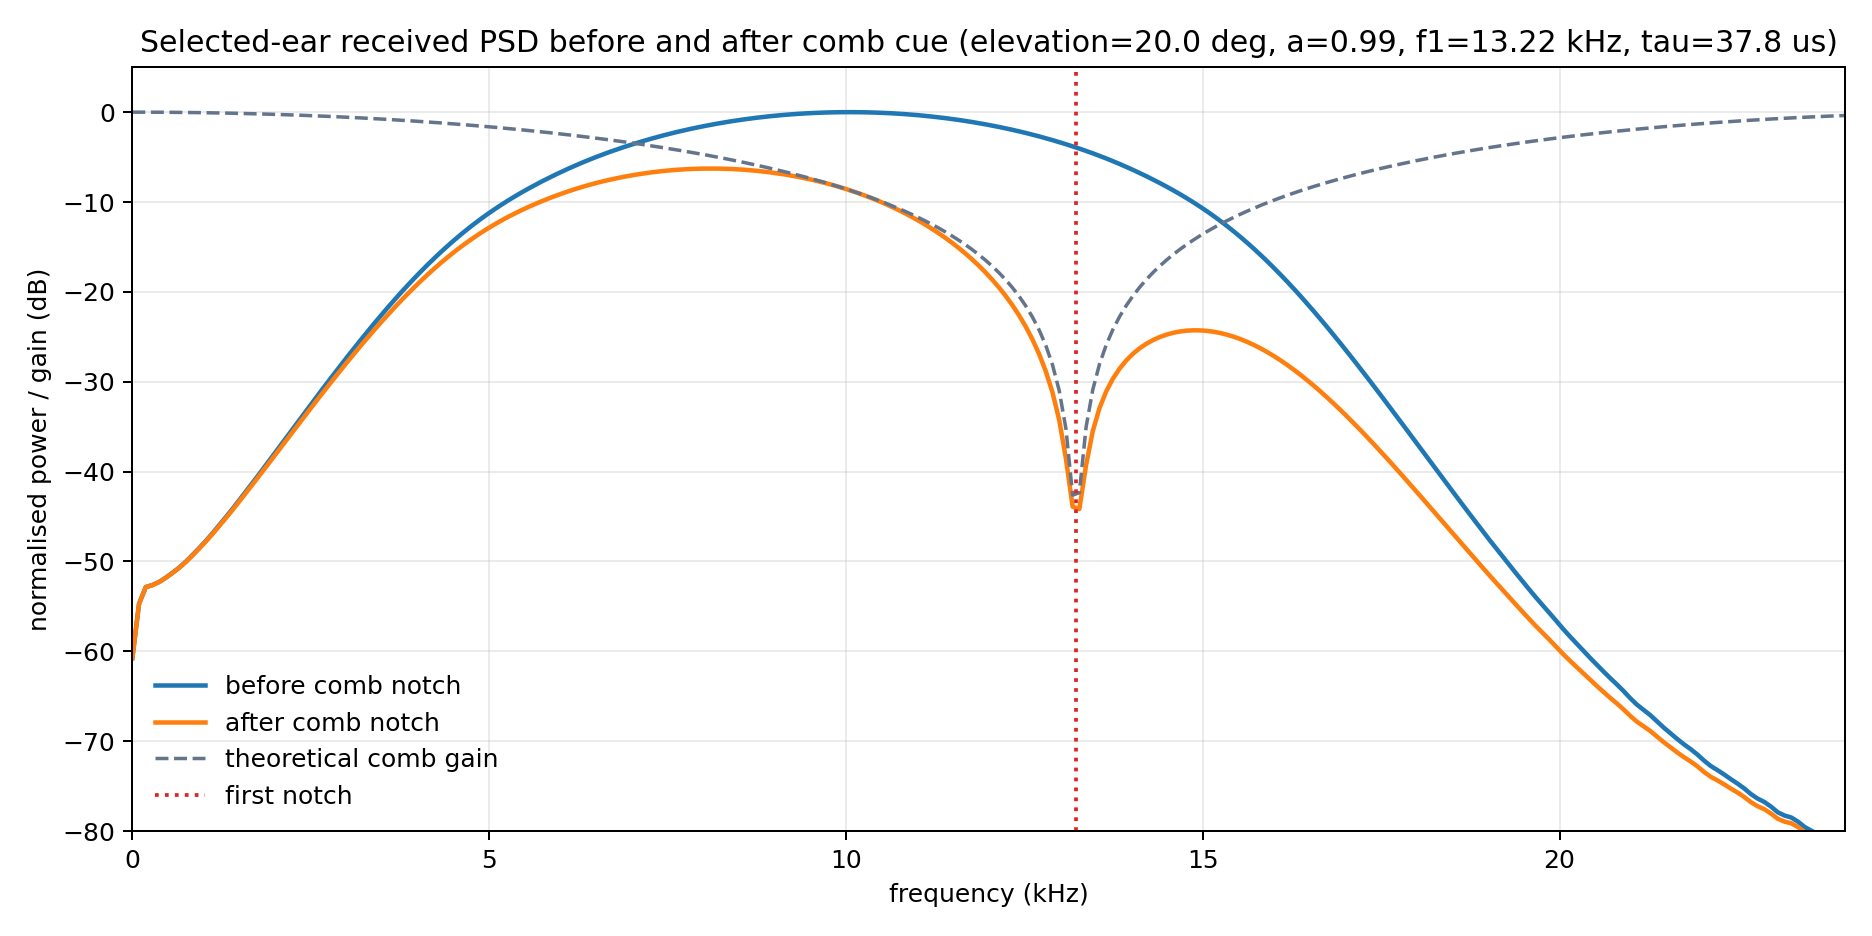
\includegraphics[width=1\textwidth]{3_Modelling/elevation/PSD.png}
    \caption{PSD of signal and comb filter across frequency channels}
    \label{fig:PSD}
\end{figure}

The mask, or what can be considered a synaptic weighting term, was adjusted to take into account the signal:
\begin{equation}
    m_k(f_c)
    =
    P_0(f_c)
    \left(
        1-H_k(f_c)
    \right)^2.
\end{equation}
This gave a high weight to frequencies where two conditions were both true: the emitted signal and cochlear front end provide useful energy, and the candidate elevation predicts a strong notch. A notch in a weak part of the spectrum should not contribute as much evidence as a notch in a high-energy part of the received call.

This weight matrix can be interpreted as a bank of fixed DCN-like spectral receptive fields. Each candidate elevation neuron receives frequency-specific synaptic weights from the cochlear channels. The known transfer function is used to set biologically plausible frequency-specific weights for a simplified notch-sensitive population, performing frequency matching without the use of FFTs. This was the signal-weighted full transfer iteration of the model.

The final improvement in the elevation experiment, the delayed-copy gain was increased to
\begin{equation}
    g = 0.99.
\end{equation}
For an ideal comb filter, the first-notch amplitude is
\begin{equation}
    |H(f_1)| = \frac{|1-g|}{1+g}.
\end{equation}
Thus, increasing $g$ makes the destructive-interference notch much deeper. This was necessary because the earlier, shallower comb cue was difficult for the downstream notch detector to recover reliably. The physical meaning of this is a pinna that is more reflective. This is not true in reality, and instead, the complex shape of the pinna creates a unique spectral fingerprint, creating an entire spectral map to use as a cue, rather than a singular notch. This notch detection is hypothesized to be a part of this expanded system, however, and so the model remains biologically grounded. 

This final iteration performed the best, with an MAE of $2.824\degree$. This was a particularly notable result as it outperformed a control reference system that used knowledge of the position of the first notch and directly calculated elevation from it. Whilst the MAE improvement was modest, the DCN model had an improved bias, and also had a maximum error of $6.49\degree$ compared to the first notch maximum error of $12.26\degree$. This was likely due to the ability of the developed model to take into account the entire response of the system, effectively having more information to infer elevation, even if the position of the notch is slightly deviated from where it should be in an ideal case. Table \ref{tab:elevation_pathway_readout_comparison} shows the performance of each of these iterations.

\begin{table}[htbp]
    \centering
    \caption{Comparison of elevation pathway readouts during development. Errors are reported in degrees over the isolated elevation test set. The selected hand-designed model was the deep-comb signal-weighted full-transfer DCN with centre-of-mass readout.}
    \label{tab:elevation_pathway_readout_comparison}
    \begin{tabular}{lrr}
        \toprule
        \textbf{Readout} & \textbf{MAE} & \textbf{Bias} \\
        \midrule
        Local-dip disinhibition COM
        & 16.907  & -9.858 \\
        Explicit E/I weight-profile COM
        & 7.099 & 2.299 \\
        Baseline-equalised full-transfer DCN COM
        & 5.181 & 2.913 \\
        Signal-weighted full-transfer DCN COM
        & 3.137 & 1.070 \\
        Deep-comb baseline-equalised full-transfer DCN COM
        & 4.837 & 2.611 \\
        \textbf{Deep-comb signal-weighted full-transfer DCN COM}
        & \textbf{2.824} & \textbf{0.814} \\
        First-notch diagnostic readout
        & 2.894 & -2.764 \\
        \bottomrule
    \end{tabular}
\end{table}

The final synaptic weights of the DCN model are shown in Figure \ref{fig:weights}. This highlights the disparity between the first notch location and where the synaptic weights focus on for inferring elevation.

\begin{figure}[h]
    \centering
    
\includegraphics[width=1\textwidth]{3_Modelling/elevation/weights.png}
    \caption{Synaptic weights of final DCN model}
    \label{fig:weights}
\end{figure}

\subsection{DCN-Inspired Refinements}

Two additional DCN-inspired mechanisms were tested as refinements: lateral inhibition across the elevation population and dynamic wideband inhibition before spectral matching. These were inspired from DCN biological inhibitory systems.

Lateral inhibition was implemented using a Mexican-hat interaction over candidate elevation neurons:
\begin{equation}
    L_{ij}
    =
    \exp
    \left(
        -
        \frac{(i-j)^2}{2\sigma_E^2}
    \right)
    -
    \gamma
    \exp
    \left(
        -
        \frac{(i-j)^2}{2\sigma_I^2}
    \right),
\end{equation}
\begin{equation}
    R'_i
    =
    \left[
        R_i + \alpha \sum_j L_{ij}R_j
    \right]_+.
\end{equation}
where $L_{ij}$ is the lateral interaction from elevation neuron $j$ to elevation neuron $i$. The first Gaussian term is the local excitatory component, with width
$\sigma_E$, and the second Gaussian term is the broader inhibitory surround, with width $\sigma_I$. The parameter $\gamma$ controls the relative strength of the inhibitory surround. In the tested model $\sigma_I > \sigma_E$, producing a Mexican-hat profile: nearby elevation neurons support each other, while more distant neurons suppress each other.

$R_i$ is the original rate-coded activity of the DCN neuron tuned to elevation bin $i$, and $R'_i$ is the laterally sharpened activity after recurrent
interaction across the elevation population. The parameter $\alpha$ controls the
overall strength of the lateral interaction. The rectification operator
$[\cdot]_+ = \max(0,\cdot)$ prevents negative firing rates.

The idea of this lateral inhibition system was to provide local cooperation and broader suppression, in order to sharpen the elevation bump without changing the cochlear evidence itself.

Dynamic wideband inhibition was implemented as a non-spiking leaky `interneuron' driven by the instantaneous total cochlear spike count:
\begin{equation}
    g_t
    =
    \beta g_{t-1}
    +
    \frac{1}{C}
    \sum_c S_{c,t},
\end{equation}
\begin{equation}
    \hat{x}_{c,t}
    =
    \frac{
        x_{c,t}
    }{
        1+\eta g_t
    }.
\end{equation}
where $g_t$ is the activity of a non-spiking wideband inhibitory interneuron at
time step $t$. The parameter $\beta$ is its leak or retention factor, so larger
$\beta$ gives a slower, longer-lasting inhibitory state. $S_{c,t}$ is the
cochlear spike output of frequency channel $c$ at time $t$, and $C$ is the total
number of cochlear channels. Thus, $\frac{1}{C}\sum_c S_{c,t}$ is the
instantaneous average cochlear population activity.

$x_{c,t}$ is the pre-inhibition cochlear activity or cochleagram value in
channel $c$ at time $t$, and $\hat{x}_{c,t}$ is the divisively normalised
activity after wideband inhibition. The parameter $\eta$ controls the strength
of this divisive gain control. When many channels are active at the same time,
$g_t$ increases and all channels are scaled down by the factor
$1+\eta g_t$. This makes the elevation detector less sensitive to overall echo
loudness and more sensitive to relative spectral shape.

This gain-control mechanism was intended to reduce sensitivity to distance-dependent echo volume while preserving relative spectral shape.

Although these ideas should work in theory, parameter sweeps of the gains of these two additions found an optimal case where the gain is 0 for both of them, and the decay rate is also 0, and so they are effectively not included, or inactive, in the final model ($\alpha=\eta=\beta=0$). These were, however, tested in a clean environment, and so a useful future work to be to retest this architecture under noise, and see if there is a trade-off between the clean, no noise accuracy, and noise robustness.

\subsection{SC Readout and Calibration}

An IC model was not implemented fully for this pathway, due to the simplification of monoaural gating based on azimuth, which could be interpreted as the role of the IC here. In realiy both DCN outputs would be converged in the IC before being passed onto the SC/

The SC, similarly to the previous pathways, is the readout for the pathway pipeline. The DCN output is a one-dimensional population over candidate elevations, and so a direct COM readout can again be used to decode this population:
\begin{equation}
    \hat{\psi}_{\mathrm{COM}}
    =
    \frac{
        \sum_k R_k\psi_k
    }{
        \sum_k R_k+\epsilon
    }.
\end{equation}

The elevation pathway should overall be interpreted as a spectral-template system. The comb filter creates an elevation-dependent notch, the DCN-like population matches the observed spectrum against candidate notch templates, and the SC stage converts the resulting population into a continuous elevation estimate.

\section{Continuous Attractor Neural Network}

The distance, azimuth, and elevation pathways each produce a one-dimensional population code. The direct COM readout is simple, but it does not model neural population dynamics or stabilisation. This COM model of the SC uses floating-point calculations that give a fixed readout once the simulation is complete. With the future objective for this to be implementable on neuromorphic hardware in the future, this is suboptimal. The fixed readout also does not allow a continuous feedback loop to occur. This means if future works wish to create a control loop, they would have to fundamentally alter this SC COM readout.

To improve this model of the SC, a finite line attractor system was implemented at the end of each pathway. This system is implementable on neuromorphic hardware, and gives a continuous readout that can give a stable constant readout based on the history of inputs it has received, rather than an end-of-simulation or time-windowed COM system. This was also implemented with the idea to add stability and hyperacuity to the readout. A COM readout is still needed to get a measurable output, however, this reading can now be taken at any time from the CANN unit.

The line attractor model developed was tested and optimised in a self-contained experiment, before adding the unit to each of the pathways as the updated SC model for each, with the only difference being the corresponding connections to the system.

\subsection{Line Attractor Dynamics}

The theory for CANNs and line attractors was discussed in Chapter \ref{ch:background}. This section includes some specific details about the system implemented. As a reminder, the system used is shown in Figure \ref{fig:cann_topographic_mapping}

\begin{figure}[htbp]
    \centering
    \begin{tikzpicture}[
        % --- Attractor Layer Styles ---
        neuron/.style={
            draw=gray!80, circle, minimum size=0.9cm, line width=1.0pt, fill=white,
            font=\small\sffamily\bfseries
        },
        activeNode/.style={
            draw=blue!80!black, circle, minimum size=0.9cm, line width=1.8pt, fill=blue!5,
            font=\small\sffamily\bfseries
        },
        % --- Input Layer Styles ---
        inputNode/.style={
            draw=gray!50, circle, minimum size=0.8cm, line width=1.0pt, fill=gray!5,
            text=gray!60, font=\small\sffamily\bfseries
        },
        activeInput/.style={
            draw=teal!80!black, circle, minimum size=0.8cm, line width=1.5pt, fill=teal!5,
            text=teal!90!black, font=\small\sffamily\bfseries
        },
        % --- Connection Styles ---
        excite/.style={-{Stealth[scale=1.1]}, line width=1.3pt, blue!80!black},
        inhibit/.style={-{Circle[open, scale=1.2]}, line width=1.3pt, red!80!black},
        feedforward/.style={-{Stealth[scale=1.1]}, line width=1.2pt, gray!70!black},
        activeFF/.style={-{Stealth[scale=1.2]}, line width=1.6pt, teal!80!black}
    ]

    % ================= LAYER 1: SENSORY INPUT PATHWAY (BOTTOM) =================
    \node (indots1) at (-4.5, -2.0) {\Large $\dots$};
    \node (in1)     [inputNode] at (-3.0, -2.0) {$I_{i-2}$};
    \node (in2)     [inputNode] at (-1.5, -2.0) {$I_{i-1}$};
    \node (in3)     [activeInput] at (0, -2.0) {$I_{i}$}; % The driving sensory input channel
    \node (in4)     [inputNode] at (1.5, -2.0) {$I_{i+1}$};
    \node (in5)     [inputNode] at (3.0, -2.0) {$I_{i+2}$};
    \node (indots2) at (4.5, -2.0) {\Large $\dots$};
    
    % Layer Label Left
    \node[anchor=east, font=\small\sffamily\bfseries, gray!80!black] at (-4.8, -2.0) {Afferent Pathway Input:};

    % ================= LAYER 2: ATTRACTOR NETWORK MANIFOLD (MIDDLE) =================
    \node (dots1) at (-4.5, 0) {\Large $\dots$};
    \node (n1)    [neuron] at (-3.0, 0) {$N_{i-2}$};
    \node (n2)    [neuron] at (-1.5, 0) {$N_{i-1}$};
    \node (n3)    [activeNode] at (0, 0) {$N_{i}$}; % The central active target node
    \node (n4)    [neuron] at (1.5, 0) {$N_{i+1}$};
    \node (n5)    [neuron] at (3.0, 0) {$N_{i+2}$};
    \node (dots2) at (4.5, 0) {\Large $\dots$};
    
    % Layer Label Left
    \node[anchor=east, font=\small\sffamily\bfseries, blue!80!black] at (-4.8, 0) {CANN Attractor Layer:};

    % --- INTER-LAYER FEEDFORWARD CONNECTIONS ---
    \draw [feedforward] (in1) -- (n1);
    \draw [feedforward] (in2) -- (n2);
    \draw [activeFF]    (in3) -- node[right, midway, font=\scriptsize\sffamily\bfseries, text=teal!80!black, align=left] {Driving\\Feed} (n3); % Highlighted target drive
    \draw [feedforward] (in4) -- (n4);
    \draw [feedforward] (in5) -- (n5);

    % --- INTRA-LAYER ATTRACTOR DYNAMICS (MEXICAN HAT) ---
    
    % 1. Self-Recurrent Excitation (Moved safely to the top loop)
    \draw [excite] (n3) to[loop above, looseness=6] 
        node[above=0.1cm, font=\scriptsize\sffamily\bfseries, text=blue!80!black] {Self-Excitation} (n3);

    % 2. Short-Range Local Excitation (To immediate horizontal neighbors)
    \draw [excite] (n3) to[bend right=30] (n2);
    \draw [excite] (n3) to[bend left=30] (n4);

    % 3. Long-Range Lateral Inhibition (To distal units)
    \draw [inhibit] (n3) to[bend right=40] node[above, pos=0.7, font=\scriptsize\sffamily\bfseries, text=red!80!black] {Lateral Inhibition} (n1);
    \draw [inhibit] (n3) to[bend left=40] (n5);


    % ================= THE EMERGENT STABILIZED ACTIVITY BUMP (TOP) =================
    
    % Manifold Reference Baseline Line
    \draw[line width=0.6pt, gray!40, dashed] (-4.8, 1.4) -- (4.8, 1.4);
    
    % Smooth Gaussian Activity Envelope
    \draw[line width=1.6pt, blue!70!black, smooth] 
        (-4.5, 1.4) .. controls (-2.0, 1.4) and (-1.2, 1.5) .. 
        (-0.8, 2.2) .. controls (-0.4, 2.9) and (-0.3, 3.0) .. 
        (0.0, 3.0)  .. controls (0.3, 3.0) and (0.4, 2.9) .. 
        (0.8, 2.2)  .. controls (1.2, 1.5) and (2.0, 1.4) .. (4.5, 1.4);
        
    % Label for the activity bump
    \node[anchor=south, font=\small\sffamily\bfseries\itshape, blue!80!black] at (0, 3.1) {Emergent Coordinate Bump $\mathcal{A}(x)$};

    \end{tikzpicture}
    \caption{Topographic mapping framework of the 1D Continuous Attractor Neural Network (CANN). Raw spatial coordinate approximations from upstream auditory pathways ($I_i$) project topographically into the recurrent attractor layer. Localized feedback networks compress this input into a single sharp Gaussian profile, tracking target position smoothly across the continuous neural manifold.}
    \label{fig:cann_topographic_mapping}
\end{figure}


The SC readout was modelled as a finite one-dimensional continuous attractor. Each upstream pathway first produces a one-dimensional population code $u$ over candidate distance, azimuth, or elevation. The attractor then transforms this input population into a smoother and more stable output bump.

The continuous-time rate dynamics are
\begin{equation}
    \tau \dot{x}
    =
    -x + Wx + Bu,
\end{equation}
where $x$ is the attractor state, $\tau$ is the membrane/time constant, $W$ is the recurrent matrix, $B$ is the input matrix, and $u$ is the upstream pathway population. The readout population is
\begin{equation}
    y = Cx.
\end{equation}

This separates the attractor into three design components:
\begin{itemize}
    \item the input matrix $B$, which determines how pathway evidence enters the attractor;
    \item the recurrent matrix $W$, which determines how the population evolves and stabilises;
    \item the output matrix $C$, which determines which part of the attractor state is decoded.
\end{itemize}

For the two-block E/I model, the state is
\begin{equation}
    x =
    \begin{bmatrix}
        x_E\\
        x_I
    \end{bmatrix},
\end{equation}
and the output matrix selects the excitatory block:
\begin{equation}
    C =
    \begin{bmatrix}
        I & 0
    \end{bmatrix},
    \qquad
    y = x_E.
\end{equation}
The inhibitory block shapes the transient dynamics, but is not itself decoded as the represented coordinate.

\subsection{Input Matrix and Fisher Information Optimisation}

The input matrix was selected using Fisher information as an analytical design criterion. The attractor simulations are deterministic, but FI was used to optimise how distinguishable nearby coordinates would be if the output population was observed with small independent readout noise:
\begin{equation}
    \tilde{y}(d,t)
    =
    y(d,t)+\epsilon,
    \qquad
    \epsilon \sim \mathcal{N}(0,\sigma_n^2 I).
\end{equation}
Under this model,
\begin{equation}
    J(d,t)
    =
    \frac{1}{\sigma_n^2}
    \left\|
        \frac{\partial y(d,t)}{\partial d}
    \right\|_2^2 .
\end{equation}
Therefore, apart from the constant scale factor $\sigma_n^{-2}$, maximising FI is equivalent to maximising the sensitivity of the output population to small changes in represented position.

For linear dynamics,
\begin{equation}
    y(d,t)
    =
    C e^{At} B h(d),
    \qquad
    A=\frac{-I+W}{\tau},
\end{equation}
so
\begin{equation}
    \frac{\partial y(d,t)}{\partial d}
    =
    C e^{At} B h'(d).
\end{equation}
This allows input matrices to be compared without fitting labels.

The tested two-block opponent input was
\begin{equation}
    B_{\mathrm{opp}}
    =
    \frac{1}{\sqrt{1+\beta^2}}
    \begin{bmatrix}
        M\\
        -\beta M
    \end{bmatrix},
\end{equation}
where $M$ is the finite-line input matrix and $\beta$ controls the relative opponent/inhibitory drive. The diagonal control used $M=I$, while the best model used a reflected Gaussian $M$ to correct finite-line boundary loss.

\begin{table}[htbp]
    \centering
    \caption{Finite-line input comparison using the two-block opponent attractor. Lower CRB RMSE indicates higher Fisher-information sensitivity.}
    \label{tab:cann_fi_input_comparison}
    \begin{tabular}{lrrrr}
        \toprule
        \textbf{Input} & \textbf{Width} & \textbf{$\beta$} & \textbf{Final CRB RMSE} & \textbf{5 ms CRB RMSE} \\
        \midrule
        Diagonal $M=I$ & 0 & 0.886 & 2.205 cm & 0.963 cm \\
        Raw Toeplitz & 3 & 0.896 & 0.952 cm & 0.431 cm \\
        Amplitude-corrected Toeplitz & 3 & 0.897 & 0.858 cm & 0.397 cm \\
        \textbf{Reflected Gaussian} & \textbf{3} & \textbf{0.897} & \textbf{0.851 cm} & \textbf{0.393 cm} \\
        \bottomrule
    \end{tabular}
\end{table}

\paragraph{Figure to put in:} Heatmaps of the diagonal and reflected Gaussian two-block input matrices, including $B_E$ and $B_I$.

\subsection{Recurrent Matrix}

The recurrent matrix provides the attractor dynamics after the input has been injected. In the balanced two-block model it is written
\begin{equation}
    W
    =
    \begin{bmatrix}
        K & -K\\
        K & -K
    \end{bmatrix},
\end{equation}
where $K$ is a local finite-line interaction matrix. Nearby bins excite each other through the positive terms, while the opponent block supplies balancing inhibition through the negative terms.

The raw, amplitude-corrected, and reflected variants discussed above are primarily variants of the input matrix $M$, not separate recurrent matrices. The recurrence itself is kept structurally fixed so that differences in performance can be attributed to the finite-line input geometry and opponent balance.

\paragraph{Figure to put in:} Recurrent matrix heatmap and eigenvalue/pseudospectrum plots for the selected balanced E/I recurrence.

\subsection{Output and Coordinate Decoding}

After the attractor state is evolved, the output population is decoded into a scalar coordinate. Two readouts were considered:
\begin{itemize}
    \item centre of mass (COM), which computes the weighted average over the full population;
    \item local COM, which computes the weighted average only near the peak.
\end{itemize}

The final model used global COM because it gave the most stable sub-bin readout. In the reflected Gaussian two-block test, global COM achieved lower error than the local population-vector readout.

\begin{table}[htbp]
    \centering
    \caption{Readout comparison for the reflected Gaussian two-block attractor.}
    \label{tab:cann_readout_comparison}
    \begin{tabular}{lrr}
        \toprule
        \textbf{Readout} & \textbf{Best time} & \textbf{Mean error} \\
        \midrule
        Global COM & 0.0 ms & 2.133 cm \\
        Local population vector & 0.0 ms & 3.997 cm \\
        \bottomrule
    \end{tabular}
\end{table}

\paragraph{Figure to put in:} Bump snapshots and error-over-time curves comparing global COM and local COM.

\subsection{Gain, Stability, and Biological Rate Limits}

The attractor gain controls how strongly recurrence amplifies the population bump. In the ideal linear model, increasing the balanced gain $\alpha'$ improves Fisher-information accuracy. For example, the final CRB RMSE fell from $0.851$ cm at $\alpha'=4$ to $0.295$ cm at $\alpha'=12$.

However, this ideal improvement is not biologically free. Larger gain increases the implied neural firing rate and therefore metabolic cost. A biological neuron also has a maximum firing rate, refractory period, and synaptic saturation. To test this, the finite-line model was re-run with simple firing-rate caps. The state was interpreted as activity around a baseline rate, and clipped to a maximum rate.

\begin{table}[htbp]
    \centering
    \caption{Effect of firing-rate caps on the selected reflected/opponent attractor.}
    \label{tab:cann_rate_caps}
    \begin{tabular}{lrrr}
        \toprule
        \textbf{Gain $\alpha'$} & \textbf{Cap} & \textbf{Capped CRB RMSE} & \textbf{Peak rate} \\
        \midrule
        4.0 & uncapped & 0.041 cm & 204.4 Hz \\
        4.0 & 100 Hz & 0.076 cm & 100.0 Hz \\
        4.0 & 55 Hz & 0.108 cm & 55.0 Hz \\
        8.0 & uncapped & 0.021 cm & 372.8 Hz \\
        8.0 & 100 Hz & 0.055 cm & 100.0 Hz \\
        8.0 & 55 Hz & 0.100 cm & 55.0 Hz \\
        12.0 & uncapped & 0.014 cm & 542.3 Hz \\
        \bottomrule
    \end{tabular}
\end{table}

This shows why gain cannot be increased indefinitely in a biologically plausible model. The linear system remains asymptotically stable because
\begin{equation}
    A=\frac{-I+W}{\tau},
\end{equation}
but stable dynamics can still produce large transient amplification. The selected model therefore treats the CANN as a stabilising population readout, not as an unlimited precision amplifier.

\paragraph{Figure to do:} Alpha sweep with and without firing-rate caps, plus peak-rate traces showing the biological cost of high gain.

\section{Trainable Fusion Network}

The fixed pathway model is interpretable, but full 3D localisation introduces interactions between cues. For example, azimuth affects which ear is more informative for elevation, elevation filtering changes the spectral balance used by ILD, and distance changes echo amplitude and therefore confidence. A small trainable SNN readout was therefore added as the final integration stage.

\begin{figure}[htbp]
    \centering
    \begin{tikzpicture}[
        % --- General Styles ---
        neuron/.style={
            draw, circle, minimum size=0.6cm, line width=0.8pt, fill=white,
            font=\tiny\sffamily\bfseries
        },
        lifNeuron/.style={
            neuron, draw=teal!80!black, fill=teal!5
        },
        intNeuron/.style={
            neuron, draw=purple!80!black, fill=purple!5 % Distinct style for non-spiking integrator
        },
        vectorNode/.style={
            draw, rectangle, minimum height=0.6cm, minimum width=2.4cm, rounded corners=2pt,
            line width=0.8pt, fill=white, font=\scriptsize\sffamily\bfseries, align=center
        },
        opNode/.style={
            draw, circle, minimum size=0.5cm, line width=0.8pt, fill=gray!10, font=\large
        },
        nobox/.style={
            rectangle, align=left, font=\scriptsize\sffamily
        },
        % --- Pathway Styles ---
        fixedPath/.style={line width=1.1pt, blue!70!black, -{Stealth[scale=1.1]}},
        trainablePath/.style={line width=1.1pt, teal!80!black, -{Stealth[scale=1.1]}},
        outputPath/.style={line width=1.1pt, black, -{Stealth[scale=1.1]}},
        gradientFlow/.style={line width=0.8pt, red!70!black, dashed, -{Stealth[scale=0.9]}},
        dots/.style={font=\large, gray}
    ]

    % =========================================================================
    % 1. BACKGROUND CONTAINER BOX (SNN Boundary)
    % =========================================================================
    \draw[draw=gray!30, fill=teal!2, fill opacity=0.15, rounded corners=6pt, line width=1.0pt] (3.4, -2.1) rectangle (10.5, 3.7);
    \node[anchor=north, font=\scriptsize\sffamily\bfseries, gray!60!black] at (6.4, 4.2) {snntorch Fusion Network ($f_{\text{SNN}}$)};

    % =========================================================================
    % 2. CACHED INPUT FEATURE VECTOR (z)
    % =========================================================================
    \node (pr)   [vectorNode, fill=blue!5]   at (0, 3.1)  {Distance\\Pop ($P_r$)};
    \node (paz)  [vectorNode, fill=blue!5]   at (0, 2.3)  {Azimuth\\Pops ($P^{\text{ITD, ILD}}_{\theta}$)};
    \node (pel)  [vectorNode, fill=blue!5]   at (0, 1.5)  {Elevation\\Pop ($P_{\psi}$)};
    \node (rcann) [vectorNode, fill=cyan!15]   at (0, 0.4)  {CANN $\hat{r}$\\readout};
    \node (acann) [vectorNode, fill=cyan!15]   at (0, -0.4) {CANN $\hat{a}$\\readout};
    \node (ecann) [vectorNode, fill=cyan!15]   at (0, -1.2) {CANN $\hat{e}$\\readout};
    \node (q)     [vectorNode, fill=gray!5]   at (0, -2.4) {Confidence\\($q$)};

    % Feature Vector z Structural Bracket
    \draw[line width=1.0pt, gray!60!black] (-1.4, 3.4) -- (-1.6, 3.4) -- (-1.6, -2.7) -- (-1.4, -2.7);
    \node[anchor=east, font=\scriptsize\sffamily\bfseries, gray!80!black, align=center] at (-1.8, 0.35) {Input\\Feature\\Vector $z$};
    \node[align=center, font=\small\sffamily\bfseries, gray!90] at (0, 4) {Feature Cached Inputs};

    % =========================================================================
    % 3. THE SNN LAYERS & NEURONS
    % =========================================================================
    
    % Hidden Layer 1 (Spiking LIF)
    \foreach \y [count=\i] in {2.5, 1.6, 0.7, -1.3} {
        \node (h1-\i) [lifNeuron] at (4.2, \y) {};
    }
    \node at (4.2, -0.2) [dots, rotate=90] {\dots};
    \node at (4.2, 3.2) [align=center, font=\tiny\sffamily\bfseries] {Hidden L1\\`snn.Leaky`\\(Spiking LIF)};

    % Hidden Layer 2 (Spiking LIF)
    \foreach \y [count=\i] in {2.5, 1.6, 0.7, -1.3} {
        \node (h2-\i) [lifNeuron] at (6.5, \y) {};
    }
    \node at (6.5, -0.2) [dots, rotate=90] {\dots};
    \node at (6.5, 3.2) [align=center, font=\tiny\sffamily\bfseries] {Hidden L2\\`snn.Leaky`\\(Spiking LIF)};

    % Output Integrator Layer (Non-spiking, 3 output tasks)
    \node (outI-1) [intNeuron] at (8.8, 1.8) {};
    \node (outI-2) [intNeuron] at (8.8, 0.0) {};
    \node (outI-3) [intNeuron] at (8.8, -1.2) {};
    \node at (8.8, 0.9) [dots, rotate=90] {\dots};
    \node at (8.8, 3.2) [align=center, font=\tiny\sffamily\bfseries, text=purple!90!black] {Output Integrator\\`snn.Leaky`\\(no reset)};

    % Temporal Mean Reduction Block
    \node (meanBlock) [vectorNode, fill=purple!5, minimum width=1.5cm, minimum height=1.0cm] at (11.5, 0) {Temporal Mean\\$\frac{1}{T}\sum_t U_{\text{out}}(t)$};

    % Scaling Block
    \node (scaler) [vectorNode, fill=teal!5, minimum width=1.0cm] at (11.5, -1.5) {Scale\\$\lambda$};


    % =========================================================================
    % 4. WEIGHT MATRIX PROJECTIONS (Linear Layers)
    % =========================================================================
    
    % Linear 1 Mesh (Input -> Hidden 1)
    \node[font=\tiny\sffamily\bfseries, teal!60!black] at (2.9, 0.8) {`Linear`};
    
    % Linear 2 Mesh (Hidden 1 -> Hidden 2)
    \foreach \i in {1,2,3,4} {
        \foreach \j in {1,2,3,4} {
            \draw[line width=0.4pt, teal!20] (h1-\i.east) -- (h2-\j.west);
        }
    }
    \node[font=\tiny\sffamily\bfseries, teal!60!black] at (5.35, -1.8) {`Linear` $W_{\text{hid2}}$};

    % Linear 3 Mesh (Hidden 2 -> Output Integrator)
    \foreach \i in {1,2,3,4} {
        \foreach \j in {1,2,3} {
            \draw[line width=0.4pt, purple!20] (h2-\i.east) -- (outI-\j.west);
        }
    }
    \node[font=\tiny\sffamily\bfseries, purple!70!black] at (7.65, -1.8) {`Linear` $W_{\text{out}}$};


    % =========================================================================
    % 5. CONNECTIONS, RESIDUAL BYPASS & SUMMATION
    % =========================================================================
    \node (sum) [opNode] at (11.5, -3) {$\oplus$};
    \node (fixedEst) [vectorNode, fill=cyan!5, minimum width=2.8cm] at (6, -3) {Hand-Designed Estimates ($\hat{y}_{\text{pathway}}$)};
    
    % Feature connections from Cache to Hidden L1
    \draw[trainablePath] (pr.east) -- (h1-1.west);
    \draw[trainablePath] (paz.east) -- (h1-1.west);
    \draw[trainablePath] (pel.east) -- (h1-2.west);
    \draw[trainablePath] (rcann.east) -- (h1-2.west);
    \draw[trainablePath] (acann.east) -- (h1-3.west);
    \draw[trainablePath] (ecann.east) -- (h1-3.west);
    \draw[trainablePath] (q.east) -- (h1-4.west);

    % Connect Integrator units to Temporal Mean block
    \draw[trainablePath, purple] (outI-1.east) -- ++(0.3,0) |- ([yshift=0.3cm]meanBlock.west);
    \draw[trainablePath, purple] (outI-2.east) -- (meanBlock.west);
    \draw[trainablePath, purple] (outI-3.east) -- ++(0.3,0) |- ([yshift=-0.3cm]meanBlock.west);

    % Mean output -> Scaler -> Summation
    \draw[trainablePath] (meanBlock.south) -- (scaler.north);
    \draw[trainablePath] (scaler.south) -- node[right, font=\tiny\sffamily\bfseries, text=teal!90!black] {$\lambda f_{\text{SNN}}(z)$} (sum.north);

    % Feed CANN streams to the hand-designed estimator block
    \draw[fixedPath] (rcann.east) -- ++(0.3, 0) |- (fixedEst.west);
    \draw[fixedPath] (acann.east) -- ++(0.3, 0) |- (fixedEst.west);
    \draw[fixedPath] (ecann.east) -- ++(0.3, 0) |- (fixedEst.west);

    % Long Residual Bypass Routing track
    \draw[fixedPath] (fixedEst.east) -- node[above, pos=0.5, font=\tiny\sffamily\bfseries, text=blue!70!black] {Residual Bypass Path} (sum.west);


    % =========================================================================
    % 6. COORDINATE RECOVERY READOUTS (Smooth analog vectors)
    % =========================================================================
    \node (ytargets) [draw=black, rectangle, rounded corners=4pt, line width=1.0pt, fill=gray!5, anchor=north, font=\small\sffamily, inner sep=6pt] at (5, -4) {
    \textbf{Final Targets } $\mathbf{y} = [ \, r_{\text{norm}}, \ \sin \theta, \ \cos \theta, \ \sin \psi, \ \cos \psi \, ]$};
    
    % Analog Membrane Potential Tracking Plot Canvas (Replacing old spike raster)
    \node (finalPlot) [nobox] at (11.0, 1.6) {};
    \begin{scope}[shift={(finalPlot.center)}]
        \draw[gray!30, line width=0.5pt] (-0.6, 0.2) -- (0.6, 0.2);
        \draw[gray!30, line width=0.5pt] (-0.6, 0.0) -- (0.6, 0.0);
        \draw[gray!30, line width=0.5pt] (-0.6, -0.2) -- (0.6, -0.2);
        % Continuous analog potential signals
        \draw[line width=0.7pt, purple] (-0.6, 0.15) .. controls (-0.3, 0.3) and (0.1, 0.1) .. (0.6, 0.25);
        \draw[line width=0.7pt, purple!70!black] (-0.6, -0.05) .. controls (-0.2, -0.15) and (0.2, 0.15) .. (0.6, -0.02);
        \draw[line width=0.7pt, purple!40!black] (-0.6, -0.25) .. controls (-0.4, -0.1) and (0.0, -0.3) .. (0.6, -0.18);
    \end{scope}
    \node[anchor=south, font=\tiny\sffamily\bfseries, text=purple!90!black, align=center] at (11.0, 2.1) {Un-reset Membrane\\Potentials $U_{\text{out}}(t)$\\(continuous)};
    
    % Structural connection lines for terminal tracking
    \draw[outputPath] (sum.south) |- (ytargets.east);
    \draw[purple!40!gray, dashed, line width=0.6pt] (9.1, 0.9) -- (finalPlot.west);


    % =========================================================================
    % 7. BACKPROPAGATION THROUGH TIME (BPTT) GRADIENT FLOWS
    % =========================================================================
    %\draw[gradientFlow] ([yshift=0.15cm]outI-1.west) -- node[above, font=\tiny\sffamily\bfseries, text=red!80!black] {BPTT Gradients} ([yshift=0.15cm]h2-1.east);
    %\draw[gradientFlow] ([yshift=0.15cm]h2-1.west) -- ([yshift=0.15cm]h1-1.east);
    %\draw[gradientFlow] ([yshift=0.15cm]h1-3.west) -- ([yshift=0.15cm]paz.east);

    \end{tikzpicture}
    \caption{Functional computational architecture of the Residual Fusion SNN. Pre-calculated features from the cached vector $z$ project through successive linear weight transformations and spiking hidden layers. The output linear layer drives non-spiking leaky integration units (no reset mechanism). The raw historical membrane values ($U_{\text{out}}$) are averaged over all operational timesteps, scaled via $\lambda$, and combined with hand-designed baseline path estimates ($\hat{y}_{\text{pathway}}$) to generate final coordinate readouts.}
    \label{fig:fusion_snn_architecture}
\end{figure}

\subsection{Cached Feature Vector}

The trainable readout receives a compact feature vector assembled from the fixed pathways:
\begin{equation}
    z =
    \left[
    P_r,\,
    P^{\text{ITD}}_{\theta},\,
    P^{\text{ILD}}_{\theta},\,
    P_{\psi},\,
    \hat{r}_{\text{CANN}},\,
    \hat{{\theta}}_{\text{CANN}},\,
    \hat{{\psi}}_{\text{CANN}},\,
    q
    \right],
\end{equation}
where $P_r$ is the raw distance population, $P^{\text{ITD}}_{\theta}$ and $P^{\text{ILD}}_{\theta}$ are the azimuth populations, $P_{\psi}$ is the raw elevation population, the hatted terms are CANN readouts, and $q$ contains confidence features such as population margins, total activation, and spike counts.

These features were cached before training. This was needed because running the acoustic simulation and all three pathways inside every training epoch would be unnecessarily slow. Caching also makes the training experiment reproducible: the same train, validation, and test feature sets can be reused while changing only the readout architecture or loss.

\subsection{Residual SNN Readout}

The preferred trainable model is a residual readout:
\begin{equation}
    \hat{y}_{\text{final}} = \hat{y}_{\text{pathway}} + \lambda f_{\text{SNN}}(z),
\end{equation}
where $\hat{y}_{\text{pathway}}$ is the hand-designed coordinate estimate, $f_{\text{SNN}}$ is a small snnTorch LIF network, and $\lambda$ is a residual scale. This is preferable to a direct trained readout because the fixed pathway model already performs the main localisation computation. The SNN only needs to learn systematic corrections.

The output target is:
\begin{equation}
    y =
    \left[
    r_{\text{norm}},\,
    \sin \theta,\,
    \cos \theta,\,
    \sin \psi,\,
    \cos \psi
    \right].
\end{equation}
Distance is normalised to the constrained operating range, while angles are represented as sine/cosine pairs to avoid discontinuities at angular boundaries.

\subsection{Uncertainty-Weighted Loss}

The three output tasks have different units and natural scales. A manually weighted loss would be arbitrary, so the readout uses learned uncertainty weighting. The loss is:
\begin{equation}
    \mathcal{L} =
    \frac{\mathcal{L}_r}{2\sigma_r^2} + \log\sigma_r
    + \frac{\mathcal{L}_a}{2\sigma_a^2} + \log\sigma_{\theta}
    + \frac{\mathcal{L}_e}{2\sigma_e^2} + \log\sigma_{\psi},
\end{equation}
where $\mathcal{L}_r$ is the distance MSE, $\mathcal{L}_a$ is the azimuth sine/cosine MSE, and $\mathcal{L}_e$ is the elevation sine/cosine MSE. The learned $\sigma$ terms allow the model to balance the tasks during training.

This final readout can be interpreted biologically as contextual integration. It does not replace the sensory pathways. Instead, it receives multiple uncertain population codes and learns how to combine them when cues disagree or are distorted. This is closer to a higher-level cortical or collicular integration role than to an end-to-end black-box neural network.


